%*********************************************************
% Federal University of Santa Catarina (UFSC)
% 
% Author:            Gabriel Mariano Marcelino
% 
% Created on:        13/12/2017
% Last modification: 08/02/2018
%*********************************************************

\documentclass[12pt]{book}

\usepackage[a4paper,left=2.5cm,right=2.5cm,top=2.5cm,bottom=2.5cm]{geometry}
\usepackage[T1]{fontenc}  
\usepackage[utf8]{inputenc} 
\usepackage[english]{babel}
\usepackage{ae}
\usepackage{graphicx}
\usepackage[hidelinks]{hyperref}
\usepackage{fancyhdr}
\usepackage{subfigure}
\usepackage{nomencl}				% Nomenclature list
\usepackage{float}
\usepackage{titlesec}
\usepackage{booktabs}
\usepackage{emptypage}
\usepackage{lettrine}				% First letter bigger in the begining of a chapter
\usepackage{tabularx}
\usepackage{enumitem}				% Custom enumerate
\usepackage[toc,page]{appendix}     % Appendix

\title{Telemetry, Tracking and Command Module of the FloripaSat Project}
\author{Gabriel Mariano Marcelino}
\date{09/02/2018}

% File metadata
\hypersetup
{
    pdfauthor	={Gabriel Mariano Marcelino},
    pdfsubject	={Telemetry, Tracking and Command Module Documentation},
    pdftitle	={Telemetry, Tracking and Command Module of the FloripaSat Project},
    pdfkeywords	={Cubesats, TTCs, Telecomunications}
}

% URLs font style
\urlstyle{same}

% First chapter page style
\titleformat{\chapter}[display]
	{\bfseries\Large}
	{\filright\MakeUppercase{\chaptertitlename} \Large\thechapter}
	{1ex}
	{\titlerule\vspace{1ex}\filleft}
	[\vspace{1ex}\titlerule]

% Header style
\pagestyle{fancy}
\fancyhf{}
\fancyhead[RO]{Telemetry, Tracking and Command Module}
\fancyhead[LE]{\nouppercase{\leftmark}}
\fancyfoot[RO]{\thepage}
\fancyfoot[LE]{\thepage}
\renewcommand{\footrulewidth}{0.5pt} 

% List of abbreviations
\makenomenclature
\setlength\nomlabelwidth{2cm}

% Bibliography style
\bibliographystyle{unsrt}

% Table cell size limit and alignment
\newcolumntype{L}[1]{>{\raggedright\arraybackslash}p{#1}}
\newcolumntype{C}[1]{>{\centering\arraybackslash}p{#1}}
\newcolumntype{R}[1]{>{\raggedleft\arraybackslash}p{#1}}

\begin{document}

\begin{titlepage}

%****************************************************
%****************************************************
%-- TITLE PAGE --------------------------------------
%****************************************************
%****************************************************
\thispagestyle{empty}

\begin{flushleft}
FLORIPASAT - TTC-DOC - REV1
\end{flushleft}

\begin{figure}[!ht]
	\begin{flushleft}
		
\includegraphics[width=5cm]{figures/floripasat.png}
	\end{flushleft}
\end{figure}

\begin{flushleft}
\Huge{\textbf{Telemetry, Tracking and Command Module of the FloripaSat Project}}
\rule[0pt]{\textwidth}{5pt}
\end{flushleft}

\vspace{0.2cm}

\begin{flushleft}
\textit{Module Documentation} \\
\textit{GSE, Federal University of Santa Catarina, Florianópolis - Brazil}
\end{flushleft}

\vfill
\vfill

\begin{flushright}
February 2018
\end{flushright}

\pagenumbering{roman}
\setcounter{page}{1}

\end{titlepage}

\cleardoublepage

%****************************************************
%****************************************************
%-- AUTHOR PAGE -------------------------------------
%****************************************************
%****************************************************

\thispagestyle{empty}

\begin{center}

\textbf{FloripaSat Project, Telemetry, Tracking and Command Module Documentation}

\textit{February, 2018}

\vspace{1cm}

\textbf{Project Manager:}

Eduardo Augusto Bezerra

\vspace{1cm}

\textbf{Author:}

Gabriel Mariano Marcelino

\vspace{1cm}

\textbf{Contributing Authors:}

Marcelo Daniel Berejuck \\
Sara Vega Martinez \\

\vspace{1cm}

\textbf{Layout:}

Gabriel Mariano Marcelino

\end{center}

\vspace{8cm}

\begin{figure}[!h]
%\begin{wrapfigure}{l}{0.25\textwidth}
	\begin{center}
		\includegraphics[width=0.25\textwidth]{figures/by-sa.eps}
	\end{center}
\end{figure}
%\end{wrapfigure}

\textcopyright\  2018 by Federal University of Santa Catarina. Telemetry, Tracking and Command Module of the FloripaSat Project. This work is licensed under the Creative Commons Attribution-ShareAlike 4.0 International License. To view a copy of this license, visit http://creativecommons.org/licenses/by-sa/4.0/.

%****************************************************
%****************************************************
%-- ABSTRACT ----------------------------------------
%****************************************************
%****************************************************

\chapter*{Abstract}

This document...

\smallskip
\noindent \textbf{Keywords:} Cubesats. Embedded systems. Telecomunications.

%****************************************************
%****************************************************
%-- TABLE OF CONTENTS -------------------------------
%****************************************************
%****************************************************
\tableofcontents

%****************************************************
%****************************************************
%-- LIST OF FIGURES ---------------------------------
%****************************************************
%****************************************************

\listoffigures
\addcontentsline{toc}{chapter}{List of Figures}

%****************************************************
%****************************************************
%-- LIST OF TABLES ----------------------------------
%****************************************************
%****************************************************

\listoftables
\addcontentsline{toc}{chapter}{Lista of Tables}

%****************************************************
%****************************************************
%-- NOMENCLATURE ---------------------------
%****************************************************
%****************************************************

\printnomenclature
\addcontentsline{toc}{chapter}{Nomenclature}

%****************************************************
%****************************************************
%-- INTRODUCTION ------------------------------------
%****************************************************
%****************************************************

\chapter{Introduction}

\pagenumbering{arabic}

\lettrine{T}{his} document is the general documentation of the Telemetry, Tracking and Command module of the FloripaSat project.

The TTC\nomenclature{\textbf{TTC}}{Telemetry, Tracking and Command.} (or TT\&C) is the communication module of the FloripaSat\cite{site} cubesat. It is responsible to make the communication between the earth (A ground station) and the satellite, and is divided in two sub-modules: Beacon and telemetry.

The beacon is a independent sub-module who transmits a periodic signal containing an identification data (ID) of the satellite and some basic telemetry data.

The telemetry sub-module is the main communication device. It has a bidirectional data link to receive telecommands from the earth and transmit all the requested data.

The telemetry sub-module is controlled by the OBDH\nomenclature{\textbf{OBDH}}{Onboard Data Handling.} module (The OBC\nomenclature{\textbf{OBC}}{Onboard Computer.} of the satellite), and the software for handling with this sub-module is under development in the OBDH module, and is not documented here.

\nomenclature{\textbf{PCB}}{Printed Circuit Board.}
\nomenclature{\textbf{USB}}{Universal Serial Bus.}

\cite{github}

The beacon executes the following tasks during its execution:

\begin{itemize}
	\item 145 MHz band antenna deployment.
	\item One-way communication (RX) with the EPS module, using the FSP protocol.
	\item Two-way communication (TX and RX) with the OBDH module, using the FSP protocol.
	\item Transmission of the beacon packets (In two protocols: NGHam and AX.25), containing the data from the EPS or the OBDH module and the satellite ID (``FLORIPASAT").
	\item When required by the OBDH module, the transmissions are stopped for an hibernation period (shutdown).
	\item In case of an critical failure of the OBDH module, or the uplink channel, the beacon activates its reception and is capable of make its own hibernation (shutdown).
\end{itemize}

\section{Module Requirements}

In the list below, the TTC module requirements for the mission are described. These requirements are nominated as TMR\nomenclature{\textbf{TMR}}{Telemetry, Tracking and Command Module Requirements.}, or Telemetry, Tracking and Command Module Requirements.

\begin{enumerate}[label=\textit{TMR \arabic*}, leftmargin=*, align=left]
	\item The FloripaSat shall have a physical device to inhibit radio frequency (RF\nomenclature{\textbf{RF}}{Radio Frequency.}) transmission.
	
	\begin{footnotesize}
		Compliance with CDS\nomenclature{\textbf{CDS}}{CubeSat Design Specification.} 3.3.9: The use of three independent inhibits is highly recommended and can reduce required documentation and analysis.	
	\end{footnotesize}
	
	\item The CubeSat will have the RF power output to the transmitting antenna input no greater than 1,5 W.
	
	\begin{footnotesize}
		Compliance with CDS 3.3.9.1.
	\end{footnotesize}
	
	\item The CubeSat will have the RF power output to the transmitting antenna input no less than 1,0 W (or 30 dBm).
	
	\begin{footnotesize}
		Defined by team analysis.
	\end{footnotesize}
	\item No CubeSats shall generate or transmit any RF signal from the time of integration into the P-POD\nomenclature{\textbf{P-POD}}{Poly-Picosatellite Orbital Deployer.} through 45 minutes after on-orbit deployment from the P-POD.
	
	\begin{footnotesize}
		Compliance with CDS.
	\end{footnotesize}
	
	\item TTC transceiver shall transmit and receive on the frequency of 437,9 Mhz.
	
	\begin{footnotesize}
		Defined by the team, based on available spectrum allocation to Amateur communication.
	\end{footnotesize}
	
	\item TTC beacon shall transmit on the frequency of 145,9 Mhz.
	
	\begin{footnotesize}
		Defined by the team, based on available spectrum allocation to Amateur communication.
	\end{footnotesize}
	
	\item TTC shall modulate and demodulate information using GFSK\nomenclature{\textbf{GFSK}}{Gaussian Frequency-Shift Keyring.}.
	
	\begin{footnotesize}
		Defined by the team.
	\end{footnotesize}
	
	\item TTC Beacon must transmit periodic beacon messages at an interval of 10
seconds, except when in hibernation or shutdown mode. Allows ground stations to track and receive satellite data even if telecommand was not sent to the satellite.
	\item TTC transceiver must receive signals from ground stations and demodulate them.
	\item TTC must interface with OBDH, exchanging encoded raw data received or to be transmitted.
	\item TTC must interface with OBDH using the SPI protocol ($@$2 KHz).
	
	\begin{footnotesize}
		Defined by the team.
	\end{footnotesize}
	
	\item TTC radio must modulate raw data received from OBDH using GFSK, prior to transmission, and demodulate received data and forward raw data to OBDH.
	\item TTC transceiver shall transmit and receive data at a baud rate of 2400 bps. Defined by the team, based on link budget analysis.
	\item TTC beacon shall transmit data at a baud rate of 1200 bps.
	
	\begin{footnotesize}
		Defined by the team, based on link budget analysis.
	\end{footnotesize}
	
	\item TTC beacon shall transmit packets using the NGHam and AX.25 protocols.
	
	\begin{footnotesize}
		Defined by the team.
	\end{footnotesize}
	
	\item A same beacon packet must be transmitted in both NGHam and AX.25 protocols.
	
	\begin{footnotesize}
		Defined by the team.
	\end{footnotesize}
	
	\item TTC must receive the batteries voltages from the EPS module at every 10 seconds.
	
	\begin{footnotesize}
		Defined by the team.
	\end{footnotesize}
	
	\item The payload from the packets transmitted by the beacon must contain at least the satellite ID ("FLORIPASAT") and batteries voltages (received from the EPS module at every 10 seconds).
	\item TTC uC must perform the antenna deployment of the VHF band antenna.
	
	\begin{footnotesize}
		Defined by the team.
	\end{footnotesize}
	
	\item Between the beacon packets transmissions, the beacon MCU and radio must operate in low power mode, to save energy.
	
	\begin{footnotesize}
		Defined by the team.
	\end{footnotesize}
	
	\item TTC PAs (Power amplifiers) must just only be activated during transmissions. When they are not in operation, they must be turned off.
	
	\begin{footnotesize}
		Defined by the team.
	\end{footnotesize}
	
	\item All the beacon critical data, like time control and antenna deployment status, must be stored in a non-volatile memory.
	
	\begin{footnotesize}
		Defined by the team.
	\end{footnotesize}
	
	\item TTC beacon must be able to receive a 24 hour shutdown command from the OBDH module.
	
	\begin{footnotesize}
		Compliance with AMSAT/IARU regulations.
	\end{footnotesize}
	
\end{enumerate}

%****************************************************
%****************************************************
%-- HARDWARE ----------------------------------------
%****************************************************
%****************************************************

\chapter{Hardware}

\lettrine{T}{he} TTC board is composed by the following main components:

\begin{itemize}
	\item MSP430F6659, as the beacon microcontroller.
	\item RF4463F30, as the radio module for the beacon and the telemetry link.
\end{itemize}

In the figure \ref{fig:ttc-board}, ...

\begin{figure}[!h]
	\begin{center}
		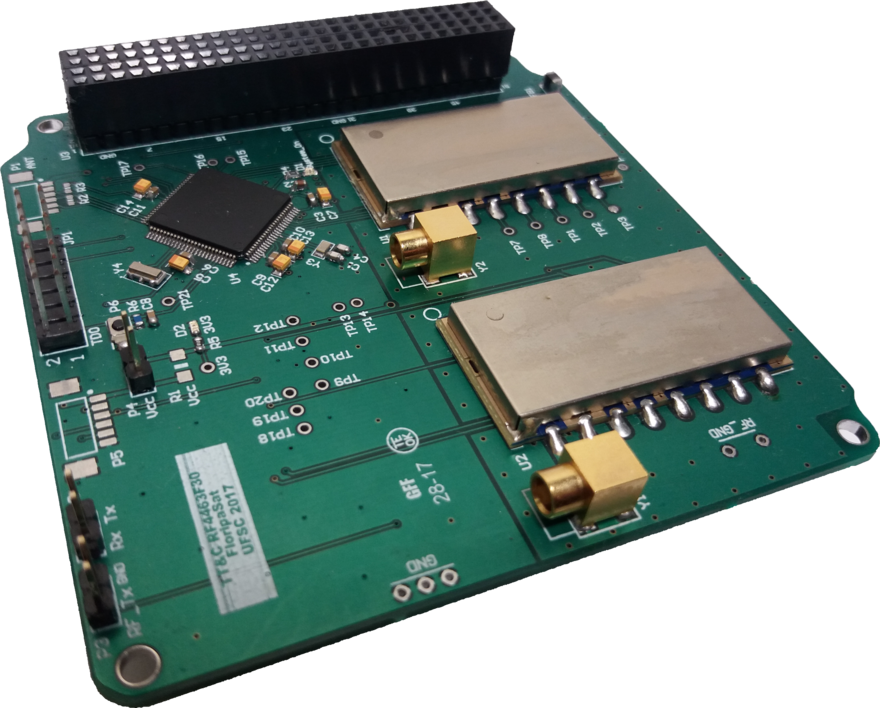
\includegraphics[width=0.75\textwidth]{figures/ttc_board.png}
		\caption{TTC PCB.}
		\label{fig:ttc-board}
	\end{center}
\end{figure}

\section{General Diagram}

In the figure \ref{fig:hardware-diagram}, a general hardware diagram can be seen, with the connection and protocols between the components.

\begin{figure}[!h]
	\begin{center}
		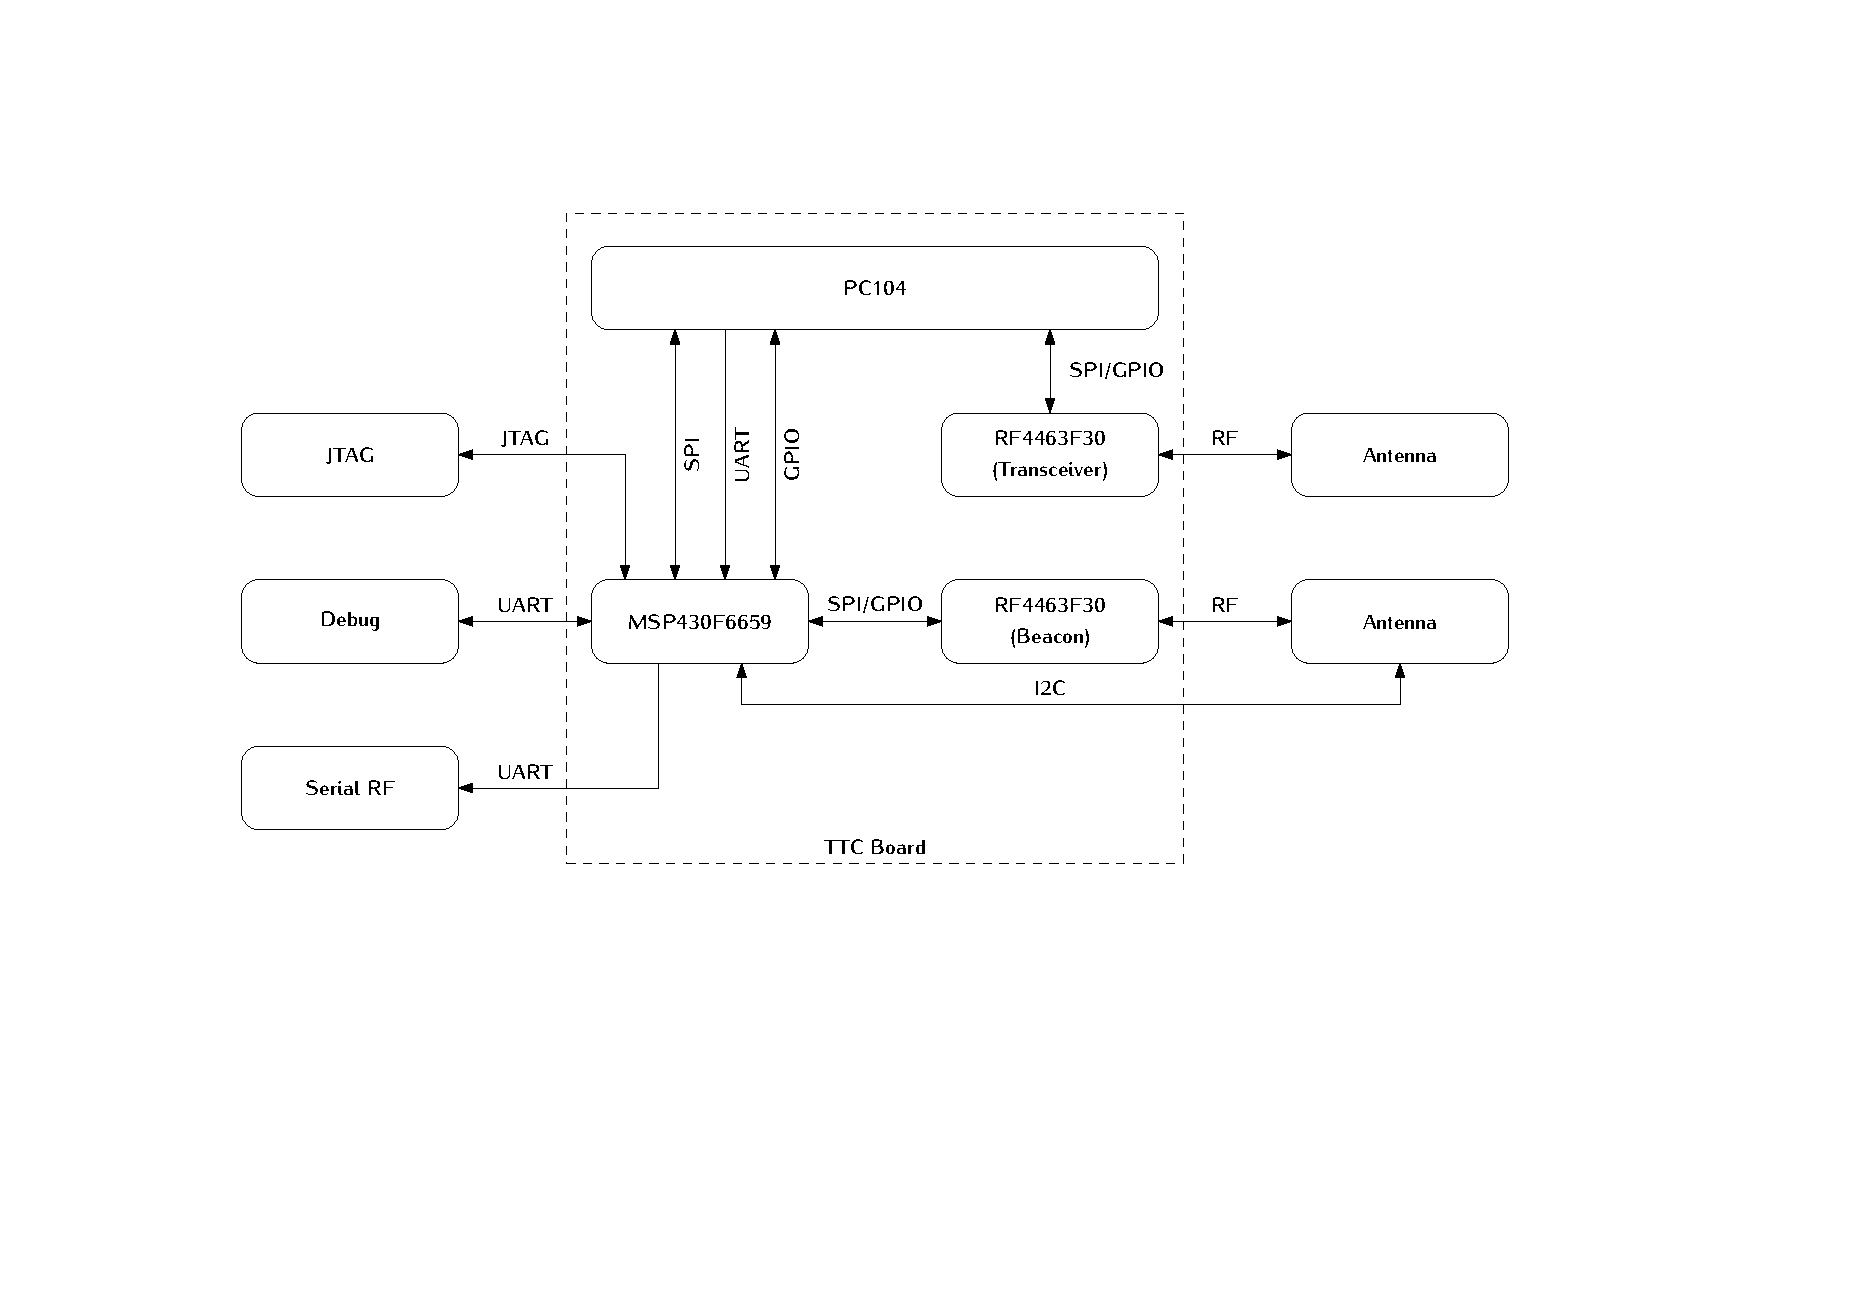
\includegraphics[width=\textwidth]{figures/hardware_diagram.pdf}
		\caption{Hardware diagram of the TTC module.}
		\label{fig:hardware-diagram}
	\end{center}
\end{figure}

\section{Main Components}

\subsection{Microcontroller}

The beacon microcontroller is the MSP430F6659IPZR \cite{msp430f6659}. Its main characteristics can be found in the table \ref{tab:msp430f6659-info}.

\nomenclature{\textbf{CPU}}{Central Processing Unit.}
\nomenclature{\textbf{RAM}}{Random Access Memory.}
\nomenclature{\textbf{GPIO}}{General Purpose Input/Output.}
\nomenclature{\textbf{I$^{2}$C}}{Inter-Integrated Circuit.}
\nomenclature{\textbf{SPI}}{Serial Peripheral Interface.}
\nomenclature{\textbf{UART}}{Universal Asynchronous Receiver/Transmitter.}
\nomenclature{\textbf{DMA}}{Direct Memory Access.}
\nomenclature{\textbf{ADC}}{Analog-To-Digital Converter.}
\nomenclature{\textbf{BSL}}{Bootstrap Loader.}

\begin{table}[!h]
	\begin{center}
		\begin{tabular}{lc}
			\toprule[1.5pt]
			\textit{Characteristic} & \textit{Value} \\
			\midrule
			CPU & MSP430 \\
			Frequency & Up to 20 MHz \\
			Non-volatile memory & 512 kB \\
			RAM & 66 kB \\
			GPIO pins & 74 \\
			I$^{2}$C & 3 \\
			SPI & 6 \\
			UART & 3 \\
			DMA & 6 \\
			ADC & ADC12-12ch \\
			Comparators & 12 inputs \\
			Timers - 16-bit & 4 \\
			Multiplier & $32 \times 32$ \\
			BSL & USB \\
			Min $V_{cc}$ & 1,8 V \\
			Max $V_{cc}$ & 3,6 V \\
			Active Power & $360\ \mu A/MHz$ \\
			Standby Power (LMP3) & $2,6\ \mu A$ \\
			Wakeup Time & $3\ \mu s$ \\
			Operating Temperature Range & -40 to 80 $^{\circ}C$ \\
			\bottomrule[1.5pt]
		\end{tabular}
		\caption{MSP430F6659 features.}
		\label{tab:msp430f6659-info}
	\end{center}
\end{table}

\subsection{Radio Modules}

The NiceRF RF4463F30 \cite{rf4463f30} is a transceiver module based on the Silicon Labs Si4463 \cite{si4463} radio. This module also contains a PA module to increase the output power up to 31 dBm.

In compliance with the \textit{TMR 3}, the RF4463F30 module operates with 5 V as input voltage in the TTC board, to achieve 30 dBm (1 W) in its output (The RF connector).

\subsubsection{Si4463}

The RF4463F30 module uses the Si4463 radio module. The main characteristics of this IC can be found in the table \ref{tab:si4463-info}.

\begin{table}[!h]
	\begin{center}
		\begin{tabular}{lcc}
			\toprule[1.5pt]
			\textit{Characteristic} & \textit{Value} & \textit{Unit} \\
			\midrule
			Frequency range & 119-1050 & MHz \\
			Receiver sensitivity & -126 & dBm \\
			Modulation & (G)FSK, 4(G)FSK, (G)MSK and OOK & - \\
			Max. output power & +20 & dBm \\
			PA support & +27 to 30 & dBm \\
			Ultra low current powerdown modes & 30 (shutdown), 50 (standby) & nA \\
			Data rate & 100 bps to 1 Mbps & - \\
			Power supply & 1,8 to 3,6 & V \\
			TX and RX FIFOs & 64 bytes for each or 129 bytes shared & - \\
			\bottomrule[1.5pt]
		\end{tabular}
		\caption{Si4463 features.}
		\label{tab:si4463-info}
	\end{center}
\end{table}

\section{External Connections}

This section describes the external available connections of the TTC module.

In the figure \ref{fig:connections-ref}, all the external connections are enumerated.

\begin{figure}[!h]
	\begin{center}
		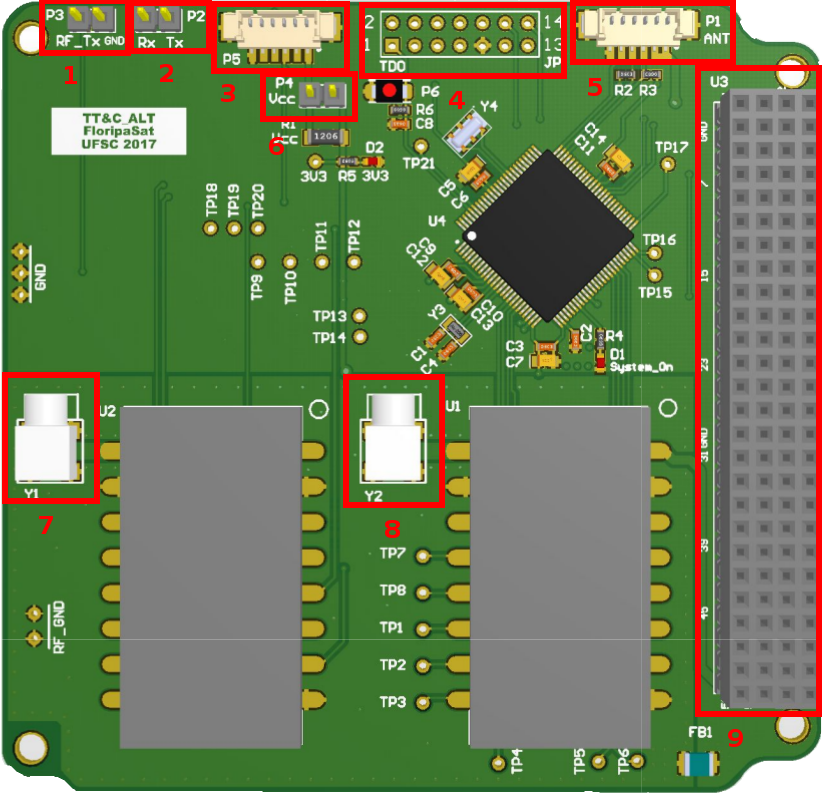
\includegraphics[width=0.75\textwidth]{figures/ttc_board_pins}
		\caption{External connections on the board.}
		\label{fig:connections-ref}
	\end{center}
\end{figure}

A brief description of each connection is presented in the table \ref{tab:connections-ref}.

\begin{table}[!h]
	\begin{center}
		\begin{tabular}{L{1.3cm} C{3cm} C{10cm}}
			\toprule[1.5pt]
			\textit{Number} & \textit{Connector} & \textit{Description} \\
			\midrule
			1 & Male pin header ($1 \times 2$) & UART TX $@$4800 bps. These pins transmit the beacon packets over a serial connection (It is enable in the configuration file, setting the BEACON\_RADIO variable as UART\_SIM). \\
			2 & Male pin header ($1 \times 2$) & Debug UART TX/RX $@$115200 bps. These pins transmit a description of the main events of the beacon software during it's execution. This feature is only available in DEBUG\_MODE. \\
			3 & Male PicoBlade$^{TM}$ ($\times 6$) & JTAG and Debug. This connection contains the relevant pins of the connectors 2 and 4. \\
			4 & Male pin header ($2 \times 2$) & MSP430 JTAG. This connection is for programming the uC code, using a MSP-FET debugger. \\
			5 & Male PicoBlade$^{TM}$ ($\times 6$) & Antenna I2C. I2C bus for a communication channel with the antenna module. \\
			6 & Male pin header ($1 \times 2$) & Power supply jumper. With a jumper, the beacon microcontroller power source comes from the JTAG connector. Without a jumper, the uC power supply comes from a pin of the PC104 connector. \\
			7 & Female Angled MCX & 437 MHz band RF signal (Goes to the antenna module). \\
			8 & Female Angled MCX & 145 MHz band RF signal (Goes to the antenna module). \\
			9 & Male/Female PCI-104 & PCI-104. Power supply and communication buses with others stacked up modules. \\
			\bottomrule[1.5pt]
		\end{tabular}
		\caption{External connections description.}
		\label{tab:connections-ref}
	\end{center}
\end{table}

The connections 1, 2, 4 and 6 were designed to be used during the software development stage, and not during the satellite operation.

\subsection{PCI-104 Pins}

The table \ref{tab:pci104-ref} describes the PCI-104 connector used pins. The first column is the row number of the connector, and the remaining columns are the respective columns (Named as H1A, H1B, H2A and H2B respectively). If the pin has no description, it is not connected to the TTC board.

\begin{table}[!h]
	\begin{center}
		\begin{tabular}{L{1cm} C{3cm} C{3cm} C{3cm} C{3cm}}
			\toprule[1.5pt]
			\textit{Row} & \textit{H1A} & \textit{H1B} & \textit{H2A} & \textit{H2B} \\
			\midrule
			1 & GND & GND & GND & GND \\
			2 & GND & GND & GND & GND \\
			3 & - & - & UART RX $@$4800 bps from the EPS module. & - \\
			4 & Telemetry radio GPIO0 & Telemetry radio GPIO1 & - & - \\
			5 & Telemetry radio GPIO2 & Enable beacon radio power supply & - & - \\
			6 & Telemetry radio SDN & - & OBDH communication (SPI MOSI) & OBDH communication (SPI clock) \\
			7 & - & - & OBDH communication (SPI chip select) & OBDH communication (SPI MISO) \\
			8 & - & - & - & - \\
			9 & - & - & - & - \\
			10 & - & - & - & - \\
			11 & - & - & - & - \\
			12 & - & - & - & - \\
			13 & - & - & - & - \\
			14 & - & - & Beacon uC power supply (3,3 V/50 mA) & 3,3 V beacon uC power supply (3,3 V/50 mA) \\
			15 & GND & GND & GND & GND \\
			16 & GND & GND & GND & GND \\
			17 & - & - & - & - \\
			18 & Telemetry radio SPI clock & - & - & - \\
			19 & Telemetry radio SPI MISO & - & - & - \\
			20 & Telemetry radio SPI MOSI & Telemetry radio SPI chip select & - & - \\
			21 & - & - & - & - \\
			22 & - & - & - & - \\
			23 & - & - & - & - \\
			24 & - & - & - & - \\
			25 & Telemetry radio power supply (5 V/500 mA) & - & - & - \\
			26 & Beacon radio power supply (5 V/500 mA) & - & - & - \\
			\bottomrule[1.5pt]
		\end{tabular}
		\caption{PCI-104 connector reference.}
		\label{tab:pci104-ref}
	\end{center}
\end{table}

\section{PCB}

The PCB (Printed Circuit Board) of the TTC module has basically the MSP430F6659 ic, the RF4463F30 module and all the external connectors.

Some characteristics of this PCB are described bellow:

\begin{itemize}
	\item The components and traces of the board are distributed over two layers (one in each side of the board).
	\item The RF modules are placed in a isolated ground plane (Connected to the main GND using a ferrite bead). This region can be seen in the figure \ref{fig:rf-ground-plane}.
	\item The antenna output of the RF4463F30 modules are connected to their respective connector over a 50 Ohm coupled trace.
\end{itemize}

\begin{figure}[!h]
	\begin{center}
		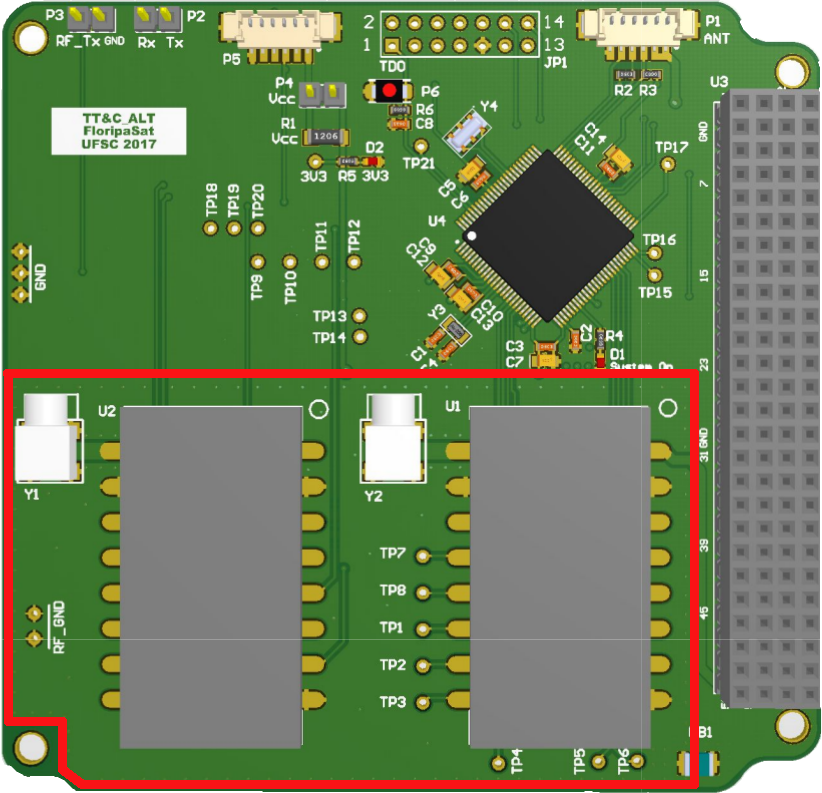
\includegraphics[width=0.5\textwidth]{figures/ttc_rf_ground_plane.png}
		\caption{RF ground plane region (red) of the TTC board.}
		\label{fig:rf-ground-plane}
	\end{center}
\end{figure}

\subsection{Types of assembly}

The TTC PCB has two types of assembly: Develop and flight.

The develop type has the purpose to be used during the development stage and tests. In this version, the connectors 3 and 5 are not soldered (Using the figure \ref{tab:connections-ref} as reference).

The flight version were designed to be used during the satellite operation. In this version, the connectors 1, 2, 4 and 6, and the reset button, are not soldered.

%****************************************************
%****************************************************
%-- SOFTWARE ----------------------------------------
%****************************************************
%****************************************************

\chapter{Software}

\lettrine{T}{he} beacon software is responsible to transmit periodic beacon signals, containing the satellite identification and a basic telemetry data.

To achieve it, this software communicates with other modules of the satellite (to acquire data to transmit in the beacon packets), controls the beacon's radio module and its antenna module.

It's written in C, using the Code Composer Studio IDE (Version 7.4.0). The radio module (Si4463 IC) is configured using the WDS (Version 3.2.11), a step-by-step tutorial is available as an apendix.

\section{Dependencies}

The beacon software is dependent of the following libraries:

\begin{itemize}
    \item NGHam: Used to generate and interpret the NGHam protocol packets (This library was modified for this firmware).
    \item DriverLib: Used to handle the internal peripherals of the MSP430F6659 uC.
\end{itemize}

\nomenclature{\textbf{HAL}}{Hardware Abstraction Layer.}

\section{Software Layers}

The figure \ref{fig:beacon-software-layers} describes the software layers of the beacon system.

\begin{figure}[!h]
	\begin{center}
		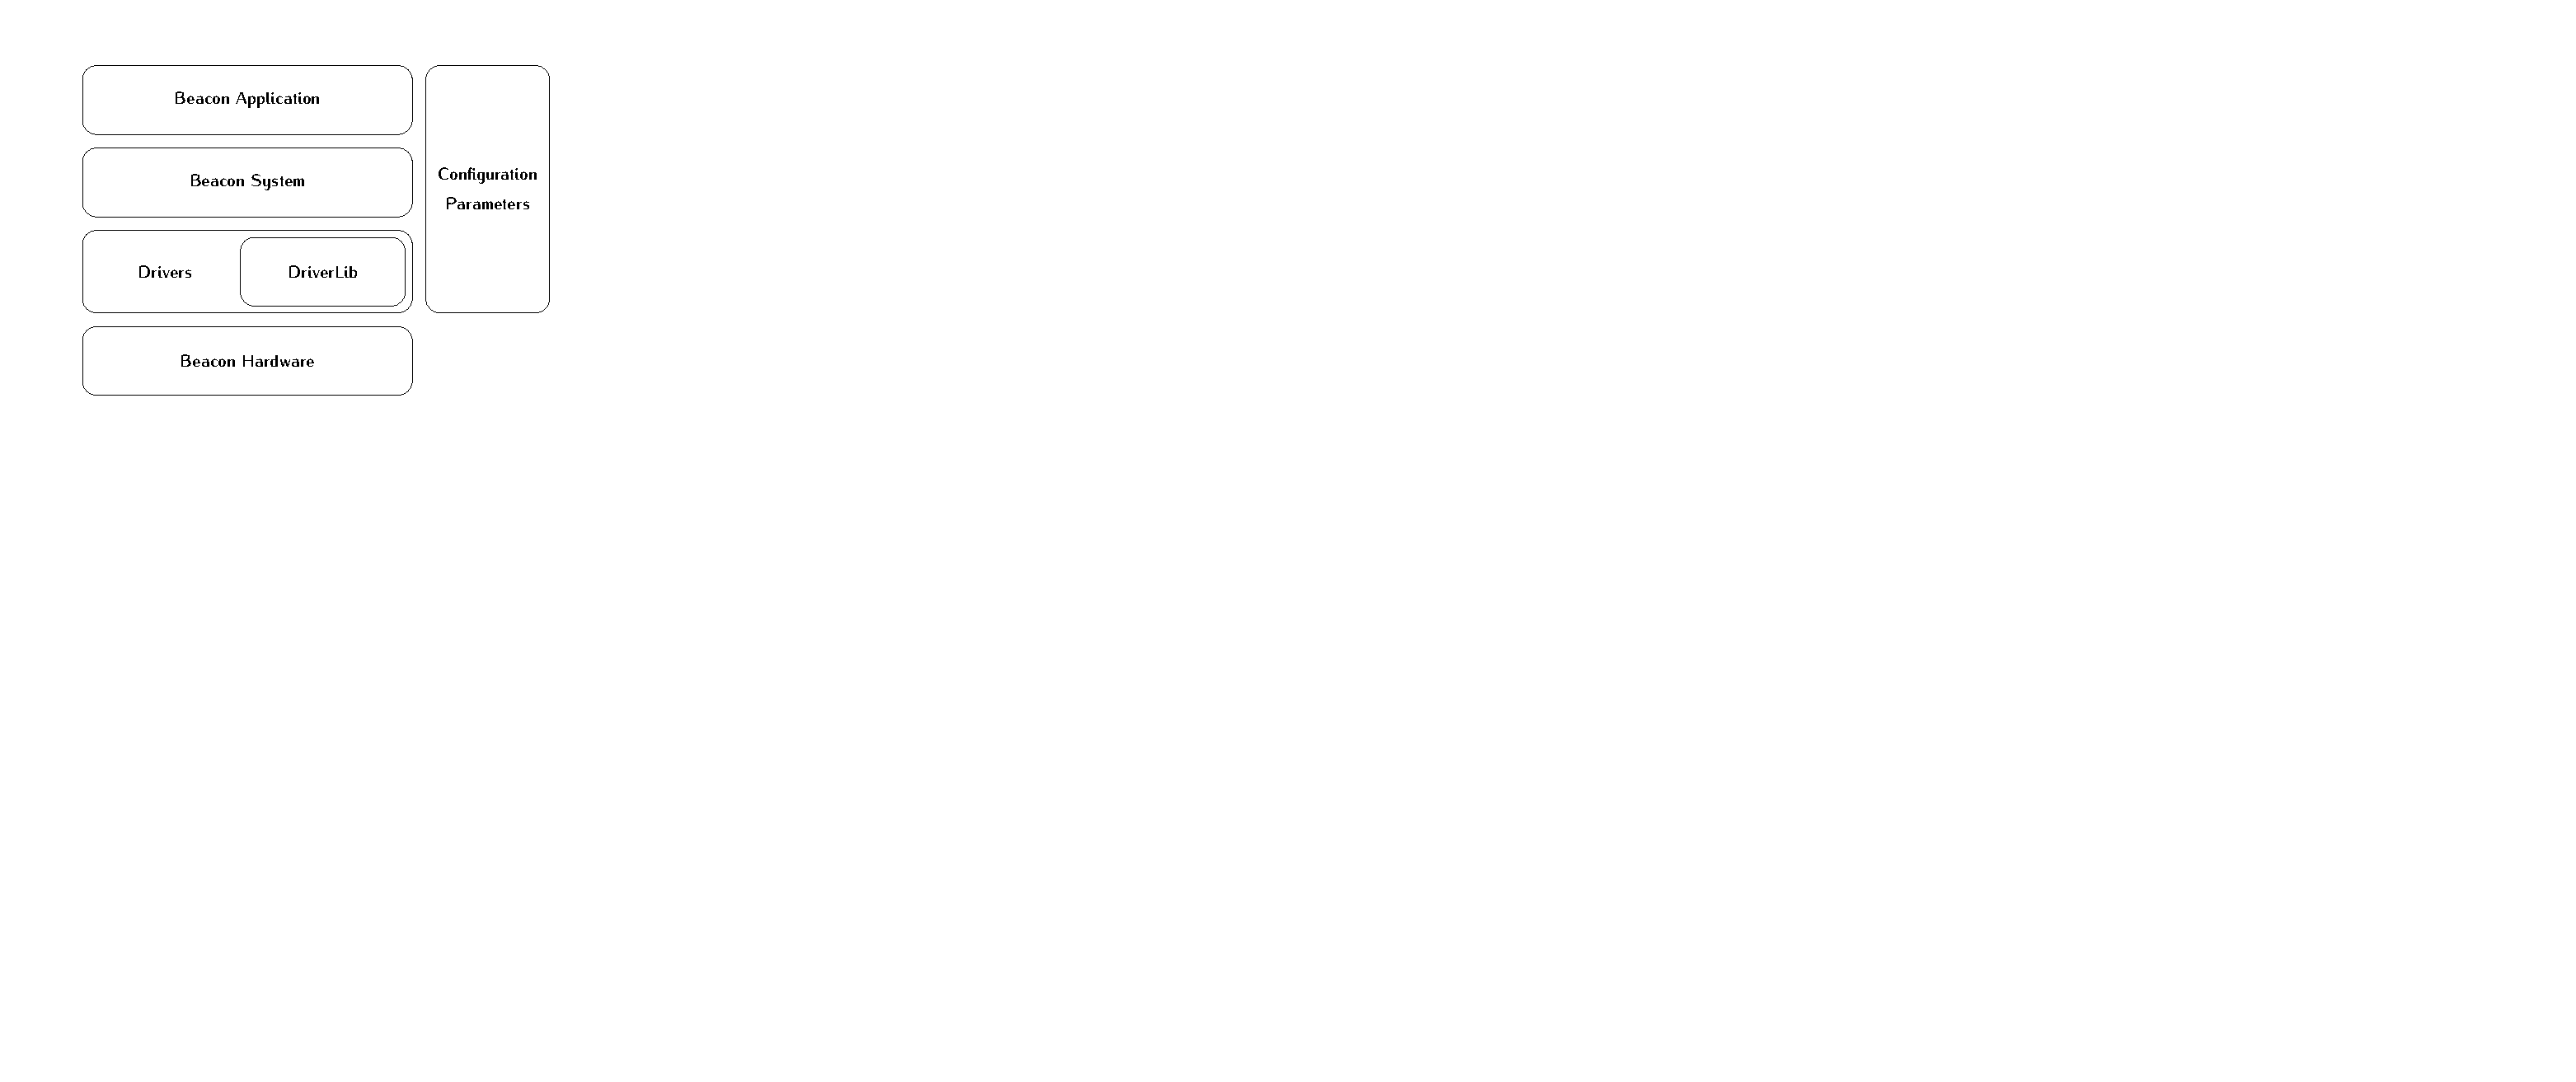
\includegraphics[width=0.5\textwidth]{figures/beacon_software_layers.pdf}
		\caption{Beacon software stack-up.}
		\label{fig:beacon-software-layers}
	\end{center}
\end{figure}

It is composed by five layers:

\begin{itemize}
    \item Hardware layer: All the TTC hardware (MSP430F6659 and the RF4463F30).
    \item Drivers layer: The software to make the interface with the hardware (Internal peripherals of the uC, the radio module and the antenna module).
    \item System layer: General usage functions and resources of the beacon system (like data structures, power management, etc.).
    \item Application layer: The main beacon software, where all the tasks were implemented.
\end{itemize}

\section{Flowcharts}

\subsection{Main}

\begin{figure}[!h]
	\begin{center}
		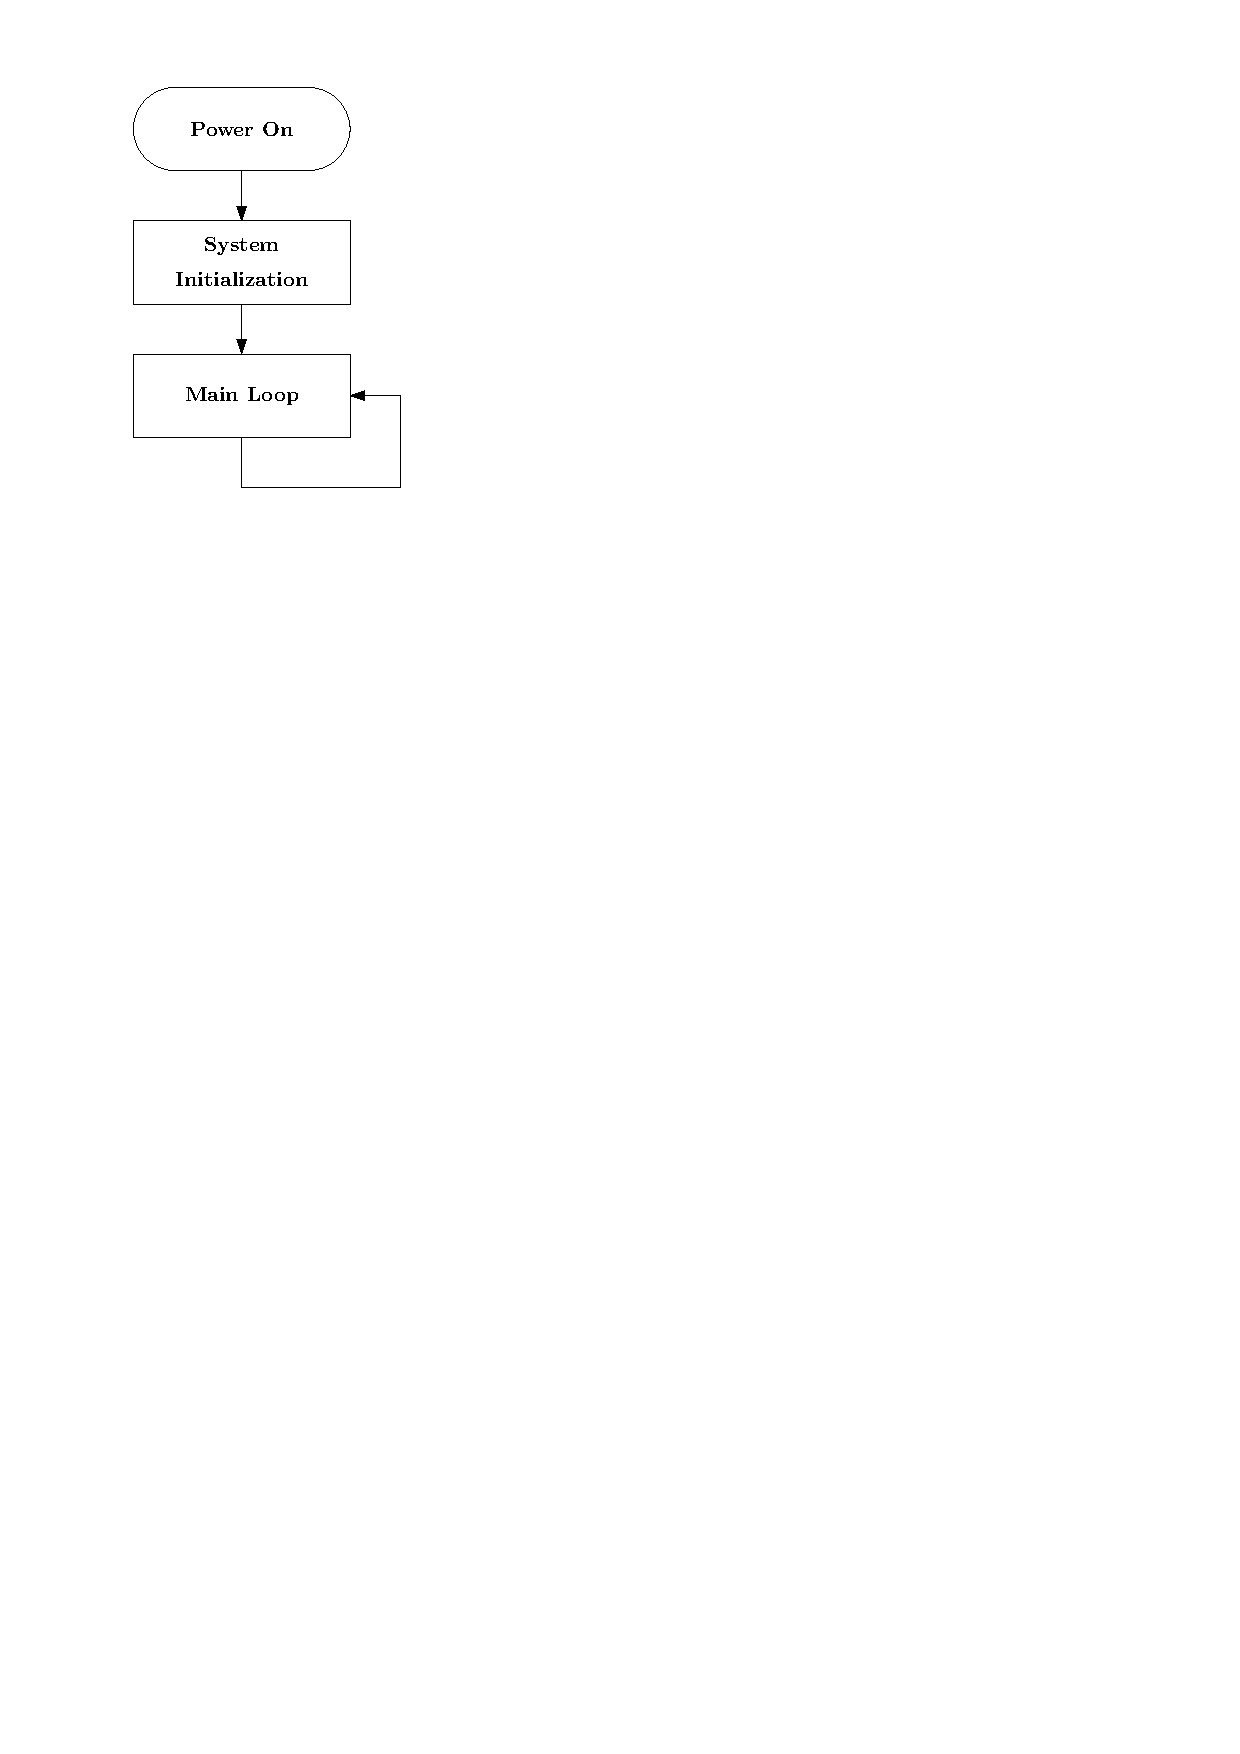
\includegraphics[width=0.25\textwidth]{figures/beacon_main_flowchart.pdf}
		\caption{Main flowchart of the beacon software.}
		\label{fig:beacon-main-flowchart}
	\end{center}
\end{figure}

\subsection{Initialization}

\begin{figure}[!h]
	\begin{center}
		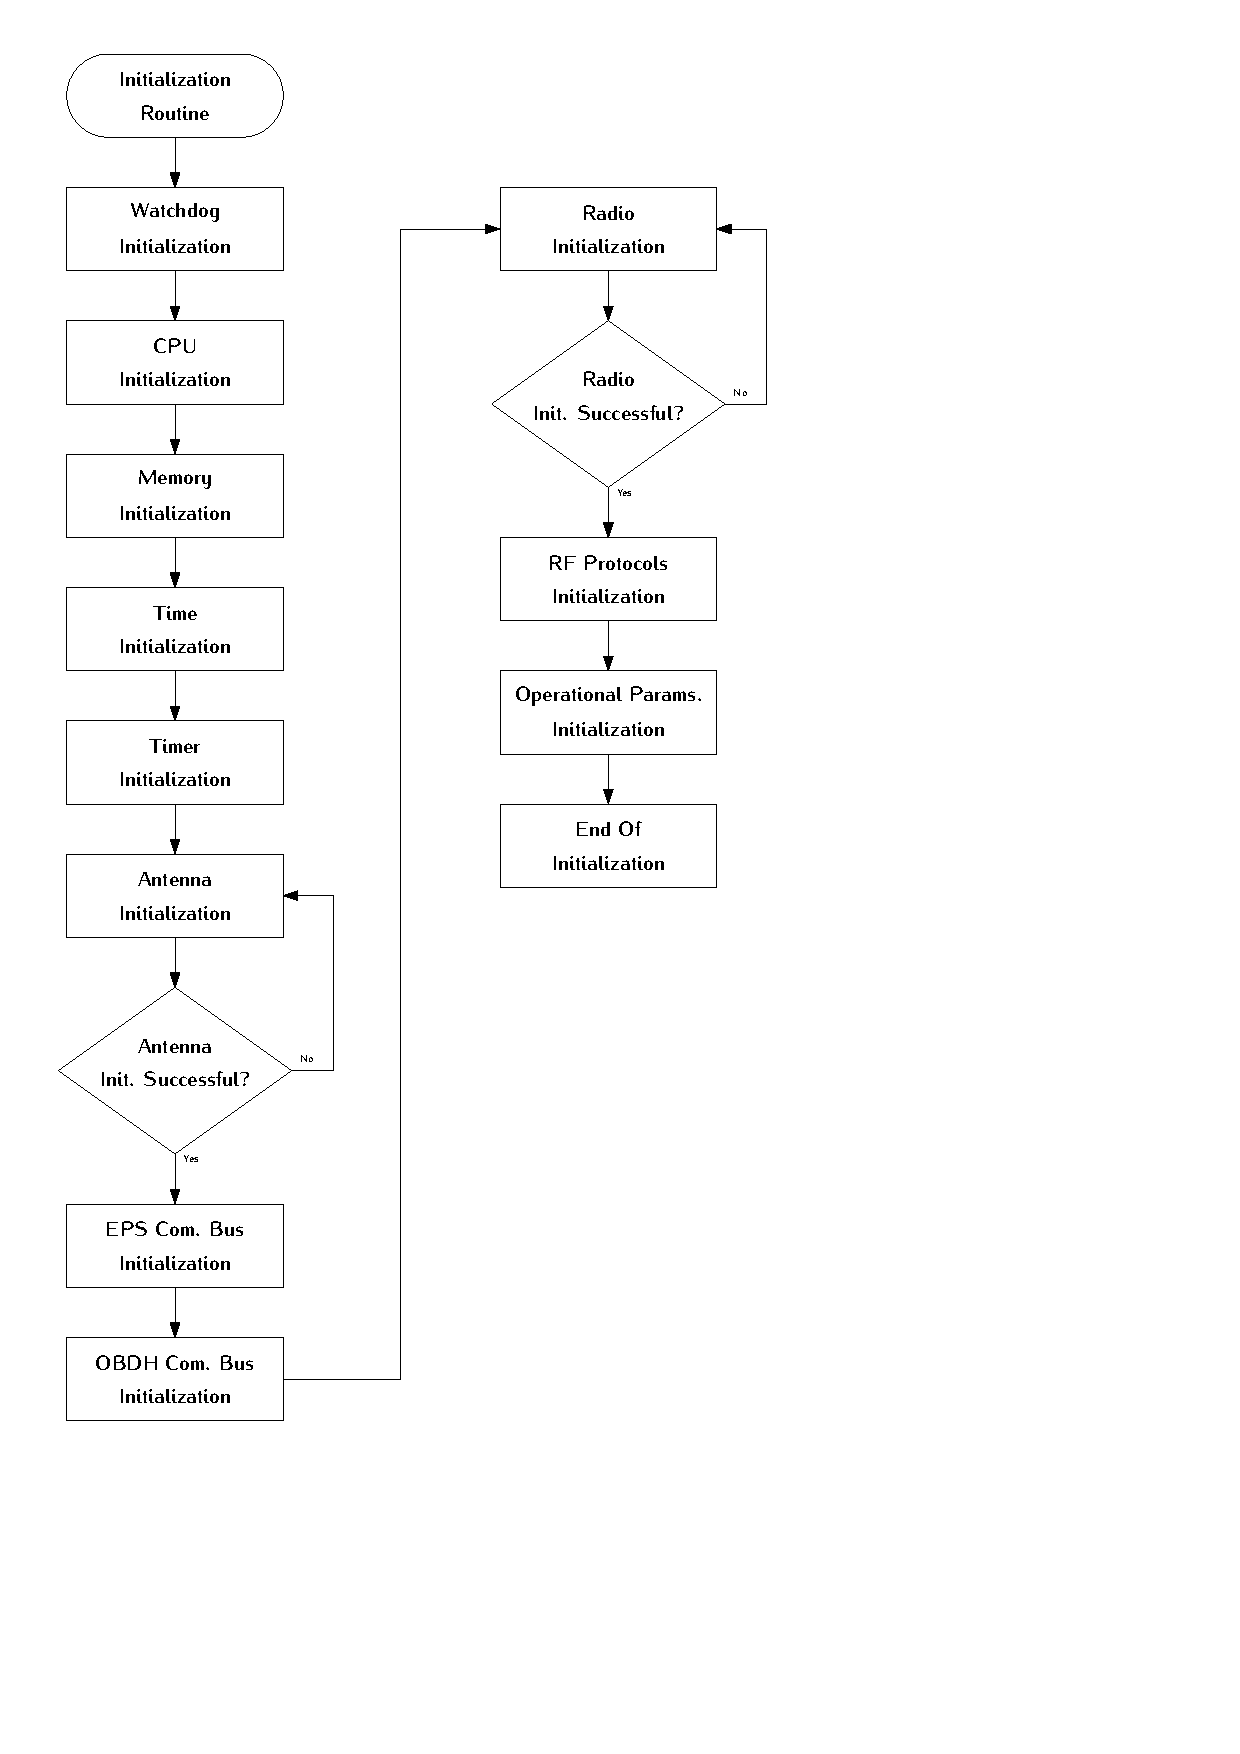
\includegraphics[width=0.75\textwidth]{figures/beacon_init_flowchart.pdf}
		\caption{Flowchart of the beacon initialization.}
		\label{fig:beacon-init-flowchart}
	\end{center}
\end{figure}

\subsubsection{Watchdog}

The watchdog is initialized using the ACLK as clock source and a 512k clock divider (generating a 16 second watchdog). The counter starts right after the initialization.

\subsubsection{CPU}

For the CPU configuration, the core voltage is setted to level 2 (required for a clock between 12 and 20 MHz). The DCO FLL reference is setted to REF0 (with the clock divider equal to 1). The ACLK clock is setted to be equal to REF0 (same as DCO, clock divider equal to 1). The SMCLK reference is setted to be the DCO, but with a divider factor equal to 4.

So, the final configuration is: MCLK = 16 MHz, SMCLK = 4 MHz and ACLK = 32,768 kHz.

\subsubsection{Memory}

UNDER DEVELOPMENT.

\subsubsection{Time}

During the time initialization, the last value stored in the memory is loaded and the counter continues from it value, preventing the lost of time reference after a system reboot or fault.

\subsubsection{Timer}

For the system time, a 1 second timer is used (using the timer interruption to increment a second counter variable, 32-bit unsigned integer). This counting starts from the last value stored into the memory.

\subsubsection{Antenna}

UNDER DEVELOPMENT.

\subsubsection{EPS Communication Bus}



\subsubsection{OBDH Communication Bus}



\subsubsection{Radio}



\subsubsection{RF Protocols}



\subsubsection{Operational Parameters}



\subsection{ISRs}

\nomenclature{\textbf{ISR}}{Interruption Service Routine.}

\subsubsection{OBDH and EPS Communication}

The flowchart of the interruption service routine (ISR) of the OBDH communication can be seen in the figure \ref{fig:beacon-obdh-isr-flowchart}. Basically, when a new byte arrives, it is pushed to a queue (if it isn't full), and periodically, the OBDH communication task process these new bytes (taking out the bytes from the queue).

The flowchart of the interruption service routine (ISR) of the EPS communication can be seen in the figure \ref{fig:beacon-eps-isr-flowchart}. It's operation is equal to the OBDH communication ISR.

\begin{figure}[!h]
	\begin{center}
		\subfigure[OBDH communication ISR flowchart.\label{fig:beacon-obdh-isr-flowchart}]{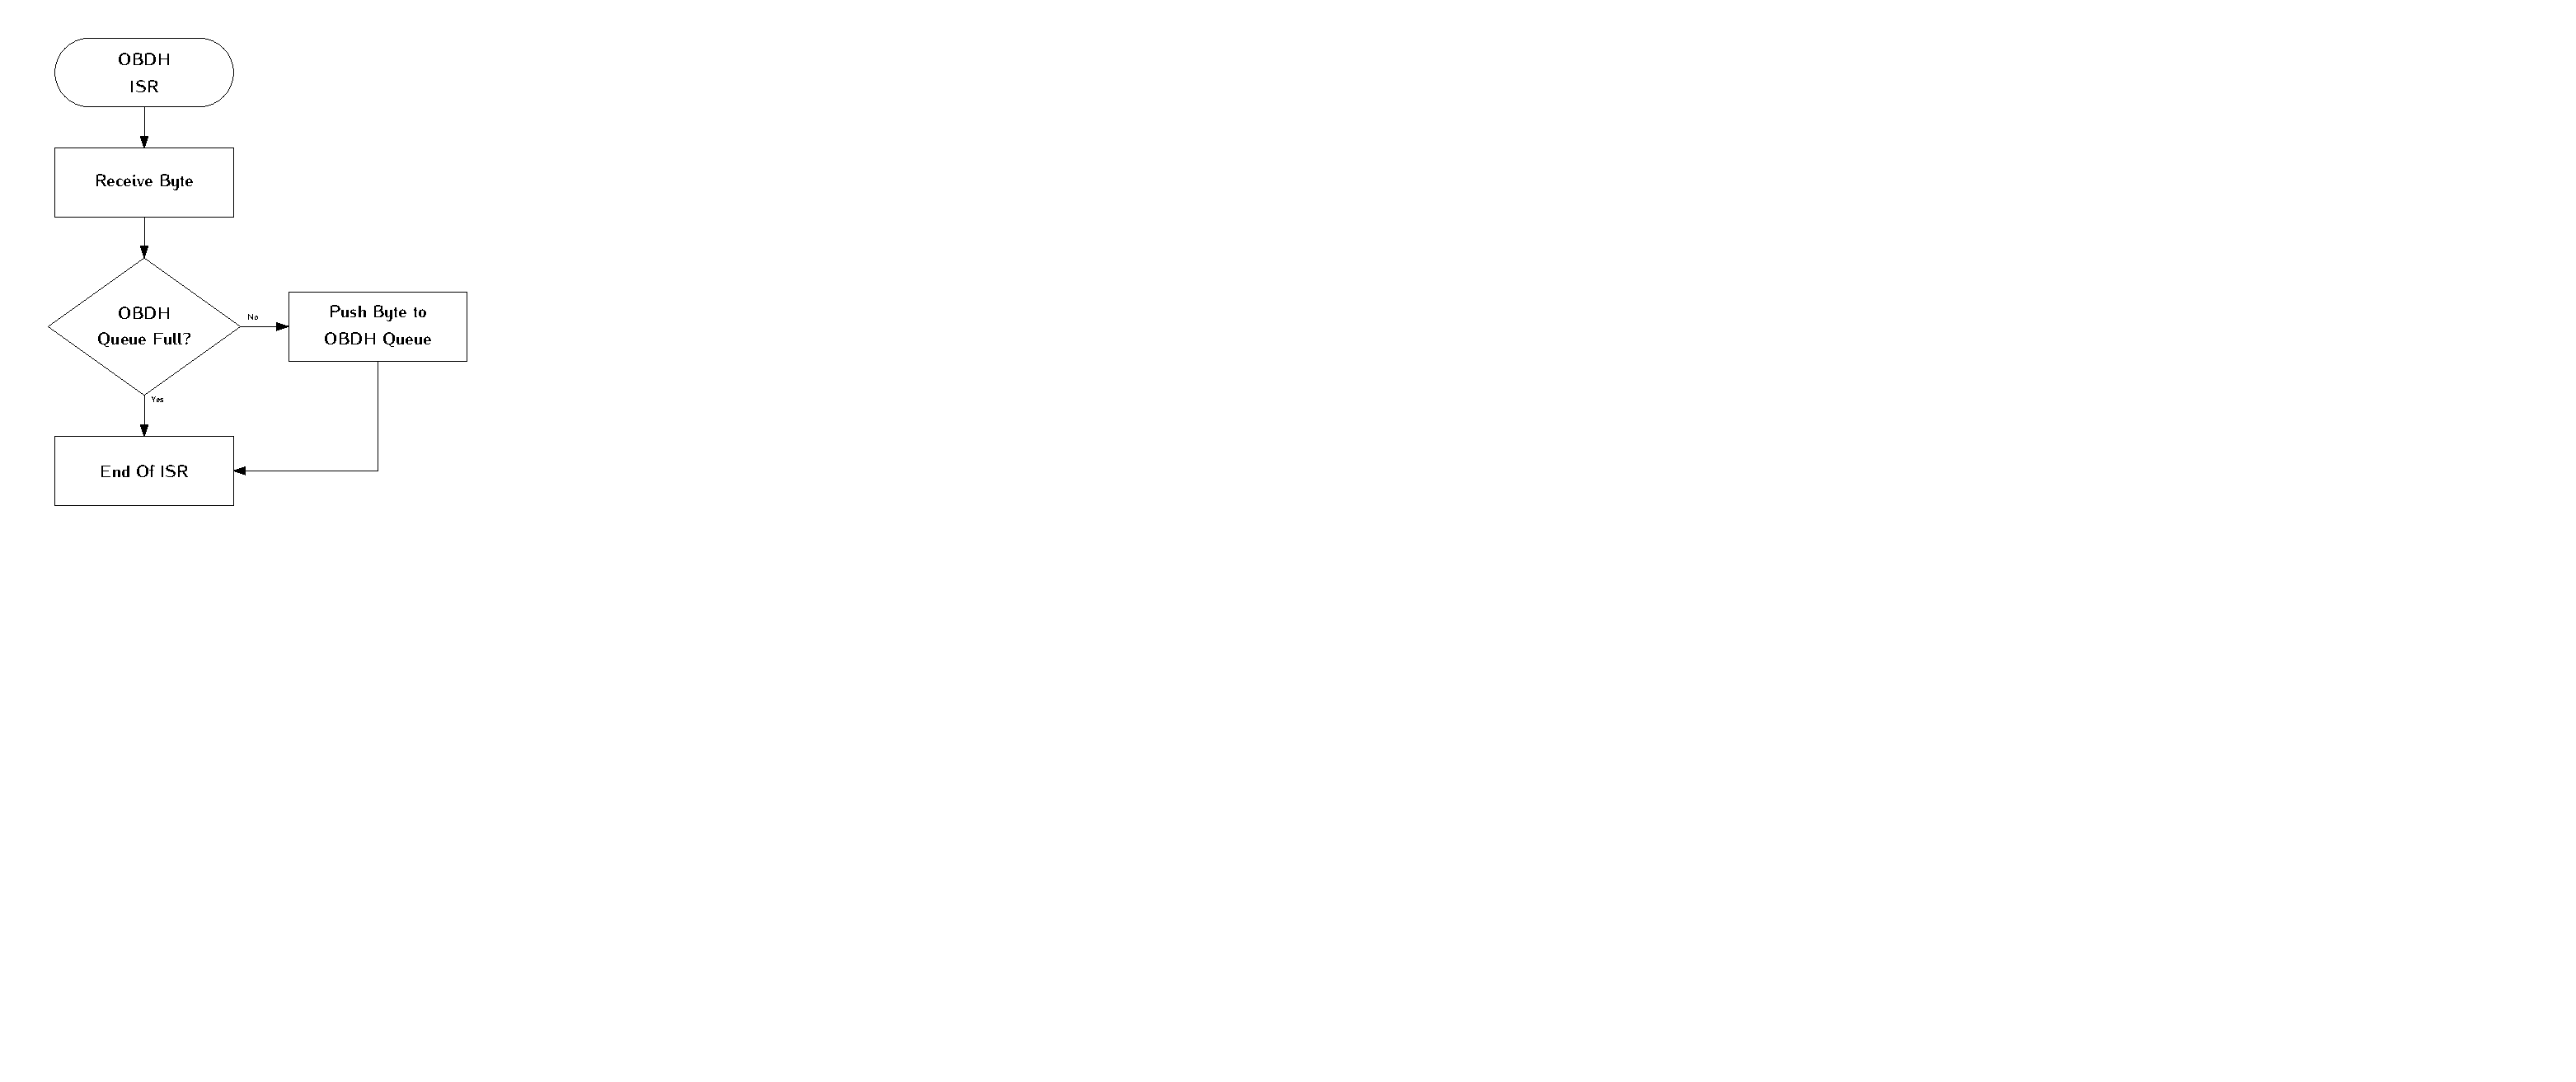
\includegraphics[width=0.4\textwidth]{figures/beacon_obdh_isr_flowchart.pdf}}
		\qquad
		\subfigure[EPS communication ISR flowchart.\label{fig:beacon-eps-isr-flowchart}]{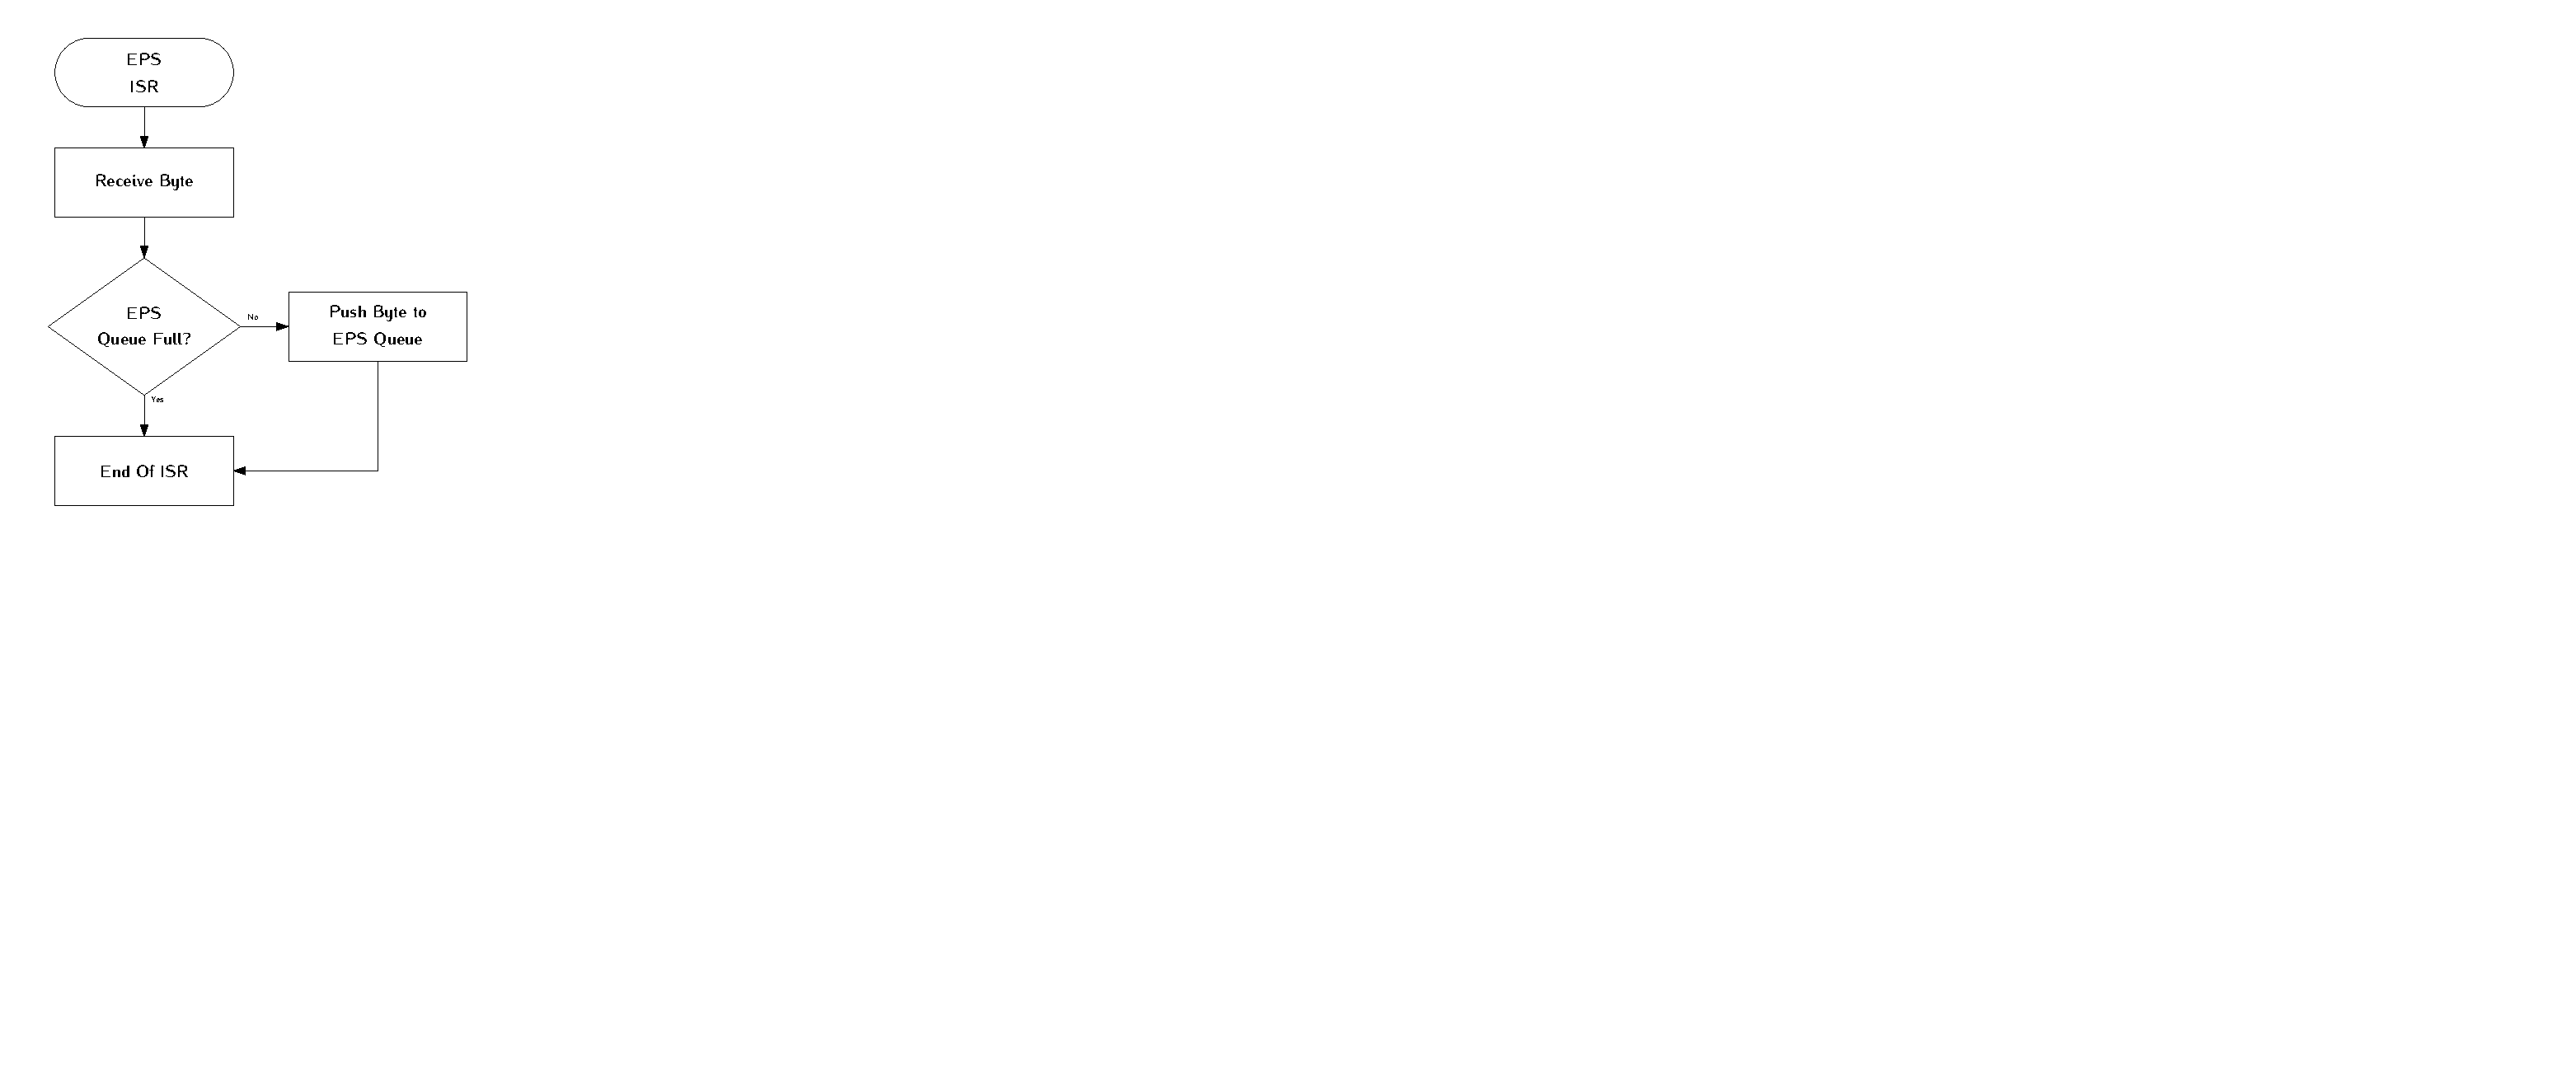
\includegraphics[width=0.4\textwidth]{figures/beacon_eps_isr_flowchart.pdf}}
		\caption{OBDH and EPS modules comunication ISRs routines.}
		\label{fig:obdh-eps-isr-flowchart}
	\end{center}
\end{figure}

\section{Operation Modes}

There are three operation modes in the beacon software:

\begin{itemize}
    \item DEBUG MODE: In this mode, the operation of the beacon is described through an UART port. At every operation, a message describing what is happening is transmitted to the debug UART port.
    \item TEST MODE: In this mode, the antenna deployment routines are not executed. This is the main mode to use during the satellite integration tests.
    \item FLIGHT MODE: This is the mode to use in flight, with all the available resources enabled.
\end{itemize}

The selection of the operation mode can be done using the ``BEACON\_MODE" variable in the ``config.h" file.

\section{Tasks}

In the table \ref{tab:sw_tasks}, the beacon tasks are listed with a brief description and its period of execution.

\begin{table}[!h]
	\begin{center}
		\begin{tabular}{L{0.2\textwidth} C{0.4\textwidth} C{0.3\textwidth}}
			\toprule[1.5pt]
			\textit{Task} & \textit{Description} & \textit{Period} \\
			\midrule
			System initialization & Submodules initialization (CPU, memory, radio, etc.) & Aperiodic (Executed only at initializations) \\
			Antenna deployment & 145 MHz band antenna deployment after the satellite launch & Aperiodic (Executed once) \\
			NGHam packet transmission & Transmission of the beacon packets with a basic telemetry data using the NGHam protocol & 10, 20 or 30 seconds (EPS energy level dependent) \\
			AX.25 packet transmission & Transmission of the beacon packets with a basic telemetry data using the AX.25 protocol & 10, 20 or 30 seconds (EPS energy level dependent) \\
			OBDH data processing & The OBDH module can send telemetry data or commands & Aperiodic (OBDH module dependent) \\
			EPS data processing & The EPS modules sends telemetry data & Aperiodic (EPS module dependent) \\
			Radio data processing & Processing of an incoming packet from the beacon radio & Aperiodic (Only when the OBDH fails and an hibernation is required) \\
			Beacon radio reception activation & When a critical failure occur in the OBDH module, the beacon activates its reception between the beacon transmissions & Aperiodic (Only when the OBDH module fails) \\
			Radio reset & Beacon radio reset & 10 minutes \\
			Beacon reset & Beacon system reset & 12 hours \\
			\bottomrule[1.5pt]
		\end{tabular}
		\caption{Beacon software tasks.}
		\label{tab:sw_tasks}
	\end{center}
\end{table}

\section{Packets Payload}

In the normal satellite operation, the beacon packets contains the data from the table \ref{tab:beacon-normal-payload}.

\begin{table}[!h]
	\begin{center}
		\begin{tabular}{lc}
			\toprule[1.5pt]
			\textit{Information} & \textit{Length (Bytes)} \\
			\midrule
			Satellite ID: ``FLORIPASAT" & 10 \\
			Batteries voltages & 4 \\
			Batteries temperatures & 6 \\
			Total charge of batteries & 2 \\
			Solar panels currents & 12 \\
			Solar panels voltages & 6 \\
			Overall status of the satellite & 2 \\
			Accelerometer and gyroscope & 12 \\
			Time since boot & 4 \\
			Number of OBDH module resets since launch & 2 \\
			\bottomrule[1.5pt]
		\end{tabular}
		\caption{Normal content of the beacon packets.}
		\label{tab:beacon-normal-payload}
	\end{center}
\end{table}

If a fault on the OBDH module occurs, only the EPS data are transmitted, the contents of this kind of packet can be seen in the table \ref{tab:beacon-without-obdh-payload}.

\begin{table}[!h]
	\begin{center}
		\begin{tabular}{lc}
			\toprule[1.5pt]
			\textit{Information} & \textit{Length (Bytes)} \\
			\midrule
			Satellite ID: ``FLORIPASAT" & 10 \\
			Batteries voltages & 4 \\
			Batteries temperatures & 6 \\
			Total charge of batteries & 2 \\
			Solar panels currents & 12 \\
			Solar panels voltages & 6 \\
			Energy level & 1 \\
			\bottomrule[1.5pt]
		\end{tabular}
		\caption{Content of the beacon packets with a fault in the OBDH module.}
		\label{tab:beacon-without-obdh-payload}
	\end{center}
\end{table}

If a fault occurs in the OBDH and the EPS modules, only the satellite ID is transmitted. It can be seen in the table \ref{tab:beacon-without-eps-payload}.

\begin{table}[!h]
	\begin{center}
		\begin{tabular}{lc}
			\toprule[1.5pt]
			\textit{Information} & \textit{Length (Bytes)} \\
			\midrule
			Satellite ID: ``FLORIPASAT" & 10 \\
			\bottomrule[1.5pt]
		\end{tabular}
		\caption{Content of the beacon packets with a fault in the OBDH and EPS modules.}
		\label{tab:beacon-without-eps-payload}
	\end{center}
\end{table}

The decodification of the packets data are done automatically by the GRS software.

\section{USCIs Configuration}

\begin{table}[!h]
	\begin{center}
		\begin{tabular}{lcc}
			\toprule[1.5pt]
			\textit{MSP Interface} & \textit{Mode} & \textit{Connected Components} \\
			\midrule
			USCI\_A0 & UART RX & EPS Bus \\
			USCI\_A0 & UART TX & Packets transmission (Only for tests) \\
			USCI\_A1 & UART TX/RX & Debug \\
			USCI\_A2 & SPI Slave & OBDH Bus \\
			USCI\_B0 & SPI Master & Beacon transceiver \\
			USCI\_B2 & $I^{2}C$ Master & Antenna bus  \\
			\bottomrule[1.5pt]
		\end{tabular}
		\caption{USCIs configuration of the beacon microcontroller.}
		\label{tab:beacon-uc-usci-config}
	\end{center}
\end{table}

\section{Timers}

\begin{table}[!h]
	\begin{center}
		\begin{tabular}{lccc}
			\toprule[1.5pt]
			\textit{Timer Interface} & \textit{Mode} & \textit{Period} & \textit{Function} \\
			\midrule
			TIMER\_A1 & Continuous-Compare & 1 s & Time Control \\
			\bottomrule[1.5pt]
		\end{tabular}
		\caption{Timers configuration of the beacon microcontroller.}
		\label{tab:beacon-uc-timers-config}
	\end{center}
\end{table}

%****************************************************
%****************************************************
%-- TESTS -------------------------------------------
%****************************************************
%****************************************************

\chapter{Tests}

\lettrine{T}{his}...

\section{RF Signal Power}

P...

%****************************************************
%****************************************************
%-- CONCLUSION --------------------------------------
%****************************************************
%****************************************************

\chapter{Conclusion} \label{ch:conclusion}

\lettrine{C}{onclusion}...

%****************************************************
%****************************************************
%-- REFERENCES --------------------------------------
%****************************************************
%****************************************************

\bibliography{references/site,references/msp430f6659,references/rf4463f30,references/si4463,references/github}
\addcontentsline{toc}{chapter}{Bibliography}

%****************************************************
%****************************************************
%-- APPENDIX ----------------------------------------
%****************************************************
%****************************************************

\begin{appendices}

\chapter{Radio Configuration}

This appendix is a tutorial with the purpose of generate a source code file with basic configuration parameters of the radio module. For it, the WDS software from Silicon Labs will be used (version 3.2.11.0).

Unfortunately, the software in only available for Windows platforms.

\section{Steps}

After the installation of the software, the procedures to configure the beacon radio are described bellow (When a parameter to configure the telemetry link radio differs from the beacon radio, a note describes the difference).

\subsection{Step 1}

\begin{enumerate}
    \item Open the WDS software.
    \item The following box will appear in the center of the window.
    \item Click in "Simulate radio" and go to the next step.
\end{enumerate}

\begin{figure}[!h]
	\begin{center}
		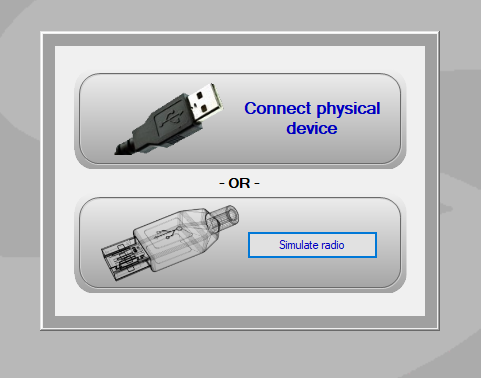
\includegraphics[width=0.5\textwidth]{figures/wds-tutorial-1.png}
		\caption{Step 1 of the radio configuration.}
		\label{fig:wds-tutorial-step-1}
	\end{center}
\end{figure}

\subsection{Step 2}

\begin{enumerate}
    \item In the list of radios that appeared on the new window, select the chip type ``Si4463".
    \item In the revision column, select ``B1".
    \item Click on ``Select Radio" to go to the next step.
\end{enumerate}

\begin{figure}[!h]
	\begin{center}
		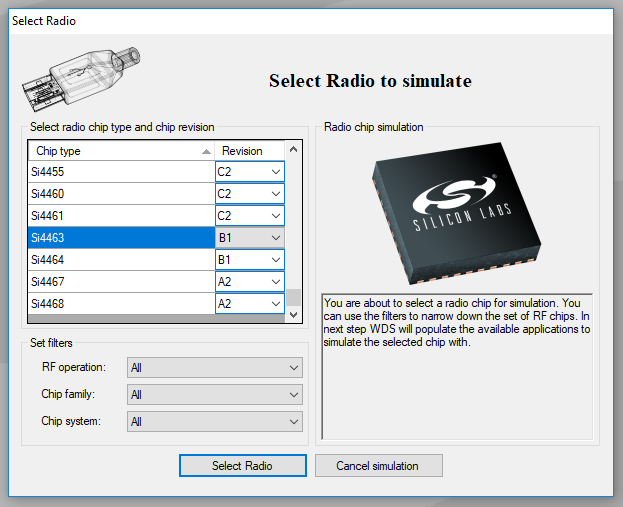
\includegraphics[width=0.75\textwidth]{figures/wds-tutorial-2.png}
		\caption{Step 2 of the radio configuration.}
		\label{fig:wds-tutorial-step-2}
	\end{center}
\end{figure}

\subsection{Step 3}

\begin{enumerate}
    \item Select ``Radio Configuration Application".
    \item Click on ``Select Application" to go to the next step.
\end{enumerate}

\begin{figure}[!h]
	\begin{center}
		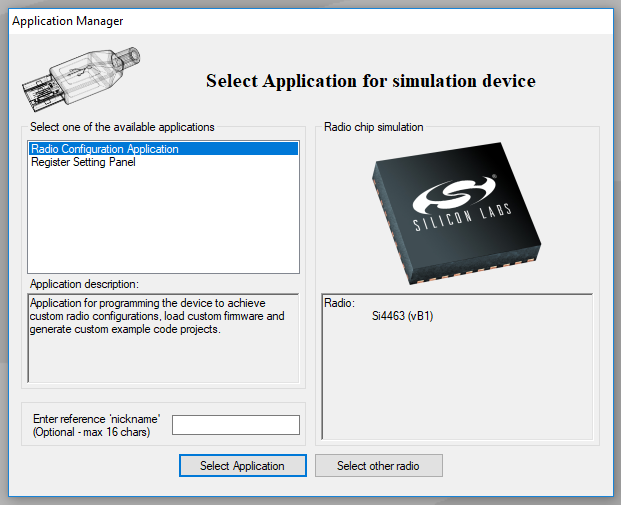
\includegraphics[width=0.75\textwidth]{figures/wds-tutorial-3.png}
		\caption{Step 3 of the radio configuration.}
		\label{fig:wds-tutorial-step-3}
	\end{center}
\end{figure}

\subsection{Step 4}

\begin{enumerate}
    \item In the ``Frequency and power" tab, change the base frequency to 145,9 MHz.
    \item Change the channel spacing to 0 kHz.
    \item Change the crystal tolerance to 10,0 ppm (Both RX and TX).
    \item Go to the next step.
\end{enumerate}

\begin{figure}[!h]
	\begin{center}
		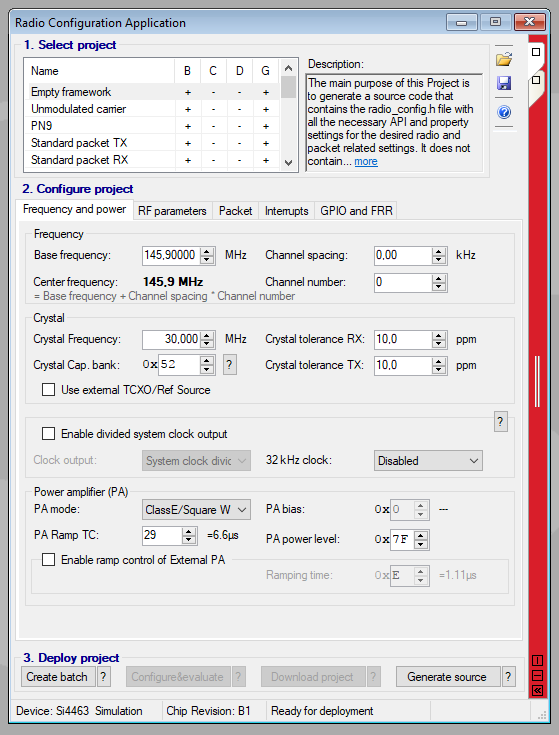
\includegraphics[width=0.75\textwidth]{figures/wds-tutorial-4.png}
		\caption{Step 4 of the radio configuration.}
		\label{fig:wds-tutorial-step-4}
	\end{center}
\end{figure}

\subsection{Step 5}

\begin{enumerate}
    \item In the ``RF parameters" tab, change the modulation type to ``2GFSK".
    \item Change the the data rate to 1,2 kbps.
    \item Change the deviation to $2,5\ kHz$.
    \item Go to the next step.
\end{enumerate}

\begin{figure}[!h]
	\begin{center}
		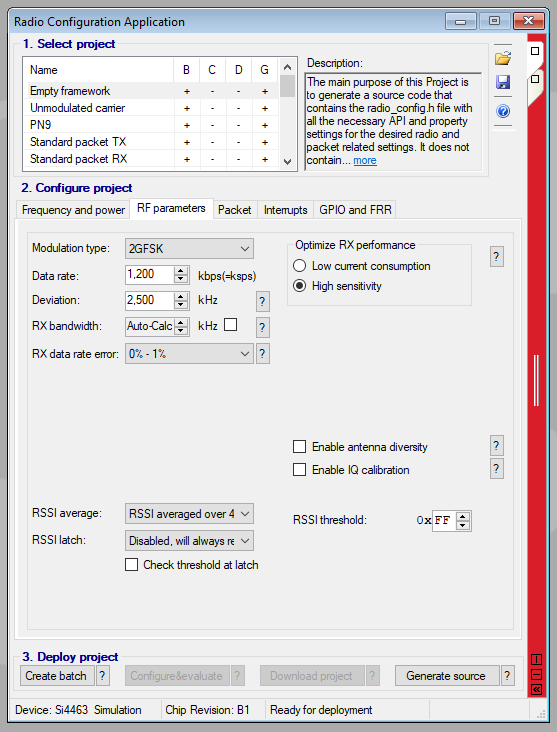
\includegraphics[width=0.75\textwidth]{figures/wds-tutorial-5.png}
		\caption{Step 5 of the radio configuration.}
		\label{fig:wds-tutorial-step-5}
	\end{center}
\end{figure}

\subsection{Step 6}

\begin{enumerate}
    \item In the ``Packet" tab, many subtabs will appear. In ``Preamble" change the ``Preamble TX length" to 4 bytes.
    \item Again, in ``Preamble", change the ``Preamble pattern" to ``Std. 1010 pattern (>= 32 and < 40 bits)".
    \item Go to the next step.
\end{enumerate}

\begin{figure}[!h]
	\begin{center}
		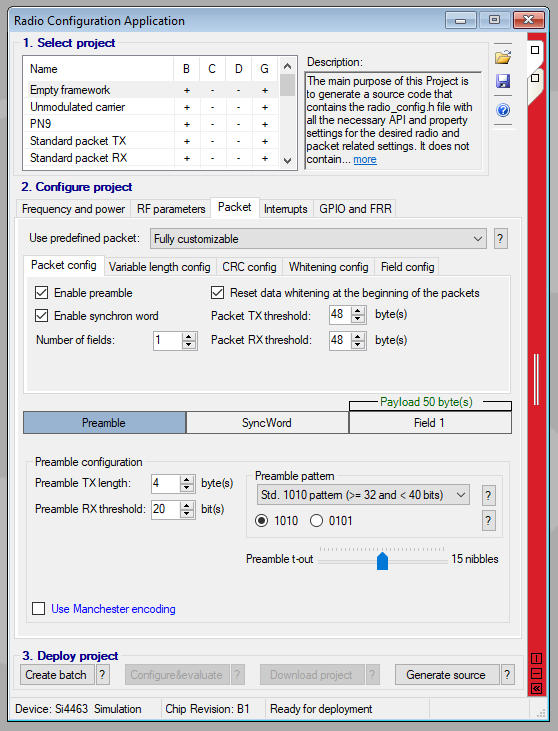
\includegraphics[width=0.75\textwidth]{figures/wds-tutorial-6.png}
		\caption{Step 6 of the radio configuration.}
		\label{fig:wds-tutorial-step-6}
	\end{center}
\end{figure}

\subsection{Step 7}

\begin{enumerate}
    \item In the ``Sync Word" tab, change the sync word length field to ``4 bytes".
    \item In the ``Sync Word (on air int.)", enter the following sequence: 5D E6 2A 7E. This sequence is the sync word used by the NGHam protocol.
    \item Go to the next step.
\end{enumerate}

\begin{figure}[!h]
	\begin{center}
		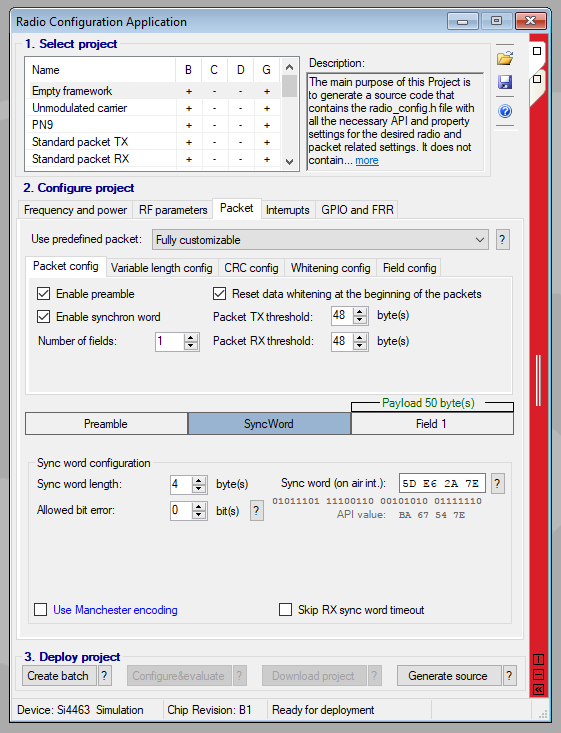
\includegraphics[width=0.75\textwidth]{figures/wds-tutorial-7.png}
		\caption{Step 7 of the radio configuration.}
		\label{fig:wds-tutorial-step-7}
	\end{center}
\end{figure}

\subsection{Step 8}

\begin{enumerate}
    \item In the ``Field 1" tab, change the ``Field length" to 50 bytes.
    \item Go to the next step.
\end{enumerate}

\begin{figure}[!h]
	\begin{center}
		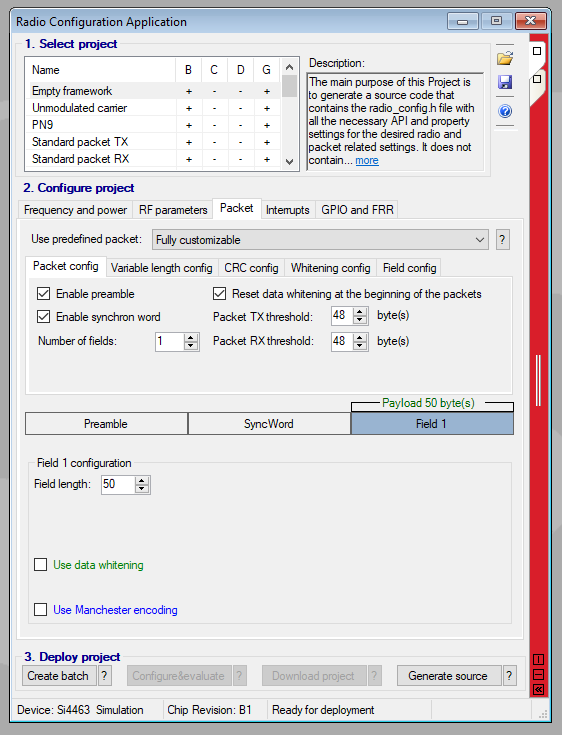
\includegraphics[width=0.75\textwidth]{figures/wds-tutorial-8.png}
		\caption{Step 8 of the radio configuration.}
		\label{fig:wds-tutorial-step-8}
	\end{center}
\end{figure}

\subsection{Step 9}

\begin{enumerate}
    \item In the ``Variable length config" tab, there is no values to change.
    \item Go to the next step.
\end{enumerate}

\begin{figure}[!h]
	\begin{center}
		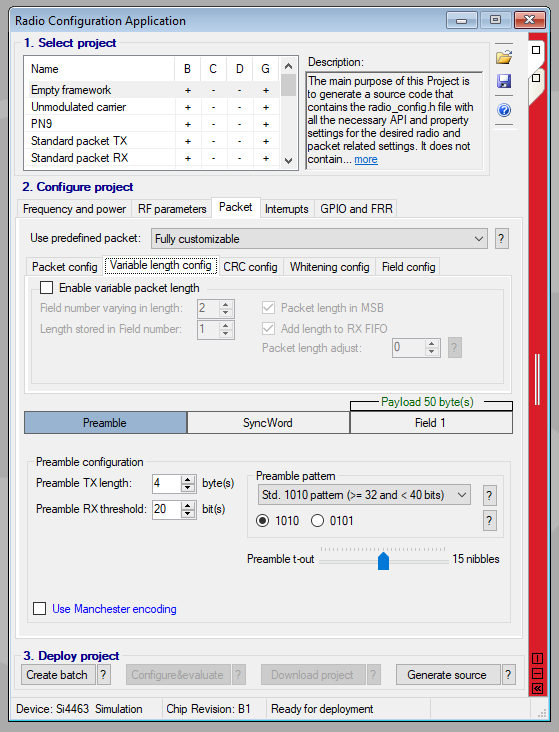
\includegraphics[width=0.75\textwidth]{figures/wds-tutorial-9.png}
		\caption{Step 9 of the radio configuration.}
		\label{fig:wds-tutorial-step-9}
	\end{center}
\end{figure}

\subsection{Step 10}

\begin{enumerate}
    \item In the ``CRC config" tab, choose ``No CRC." in ``CRC polynomial".
    \item Go to the next step.
\end{enumerate}

\begin{figure}[!h]
	\begin{center}
		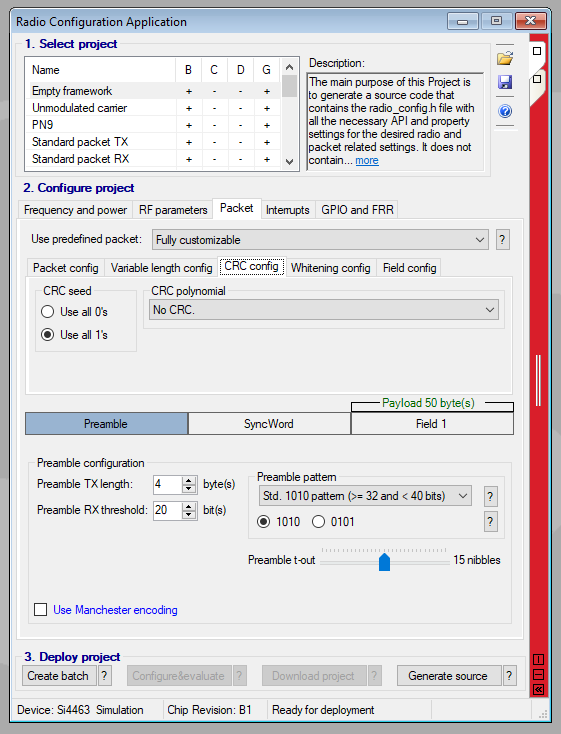
\includegraphics[width=0.75\textwidth]{figures/wds-tutorial-10.png}
		\caption{Step 10 of the radio configuration.}
		\label{fig:wds-tutorial-step-10}
	\end{center}
\end{figure}

\subsection{Step 11}

\begin{enumerate}
    \item In the ``Whitening config" tab, there is no values to change.
    \item Go to the next step.
\end{enumerate}

\begin{figure}[!h]
	\begin{center}
		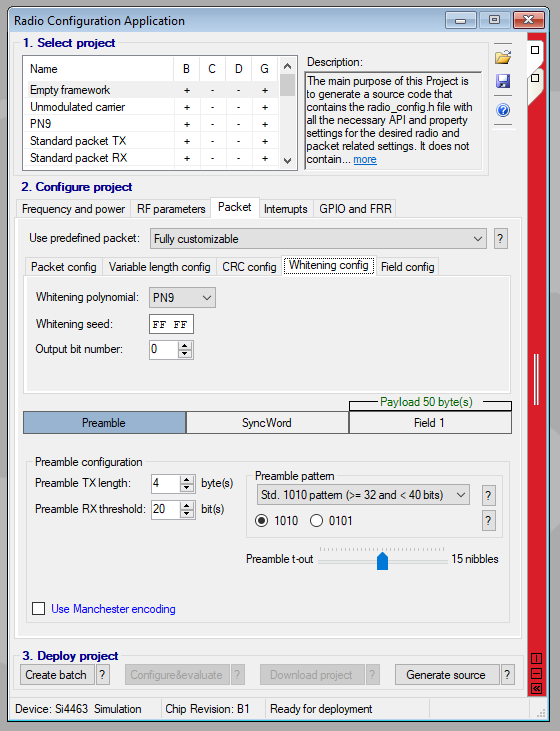
\includegraphics[width=0.75\textwidth]{figures/wds-tutorial-11.png}
		\caption{Step 11 of the radio configuration.}
		\label{fig:wds-tutorial-step-11}
	\end{center}
\end{figure}

\subsection{Step 12}

\begin{enumerate}
    \item In the ``Field config" tab, there is no values to change.
    \item Go to the next step.
\end{enumerate}

\begin{figure}[!h]
	\begin{center}
		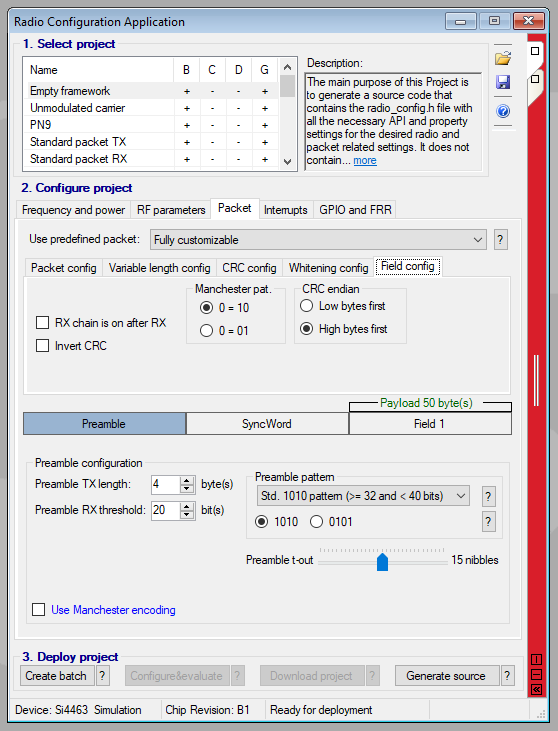
\includegraphics[width=0.75\textwidth]{figures/wds-tutorial-12.png}
		\caption{Step 12 of the radio configuration.}
		\label{fig:wds-tutorial-step-12}
	\end{center}
\end{figure}

\subsection{Step 13}

\begin{enumerate}
    \item In the ``Interrupts" tab, there is no values to change.
    \item Go to the next step.
\end{enumerate}

\begin{figure}[!h]
	\begin{center}
		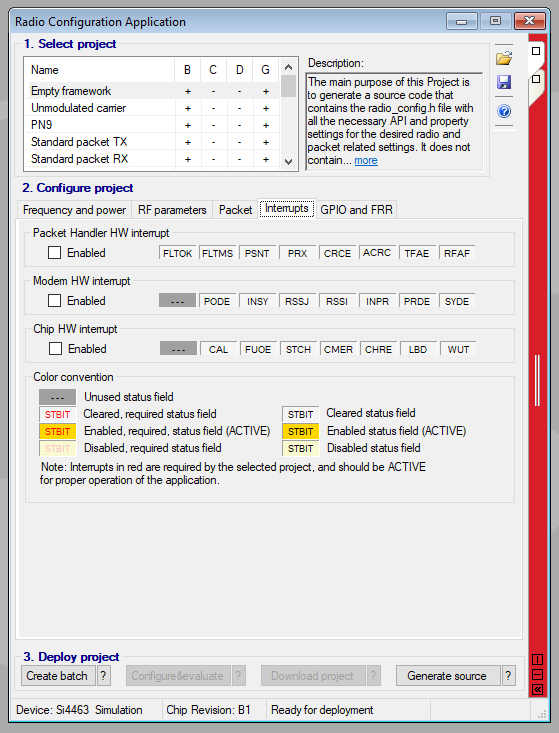
\includegraphics[width=0.75\textwidth]{figures/wds-tutorial-13.png}
		\caption{Step 13 of the radio configuration.}
		\label{fig:wds-tutorial-step-13}
	\end{center}
\end{figure}

\subsection{Step 14}

\begin{enumerate}
    \item In the ``GPIO and FRR" tab, enable pullup in GPIO1 and choose ``TX\_FIFO\_EMPTY - This output is..." as functionality.
    \item Enable pullup in GPIO2 and choose ``RX\_STATE - This output is..." as functionality.
    \item Enable pullup in GPIO3 and choose ``TX\_STATE - This output is..." as functionality.
    \item Enable pullup in NIRQ and choose ``Active low interrupt signal" as functionality.
    \item Enable pullup in SDO and choose ``SDO - Output SPI Serial data out." as functionality.
    \item Select ``Global status" for the ``Fast Response Register A".
    \item Select ``Global interrupt status" for the ``Fast Response Register B".
    \item Select ``Packet Handler status" for the ``Fast Response Register C".
    \item Select ``Chip status status" for the ``Fast Response Register D".
    \item Go to the next step.
\end{enumerate}

\begin{figure}[!h]
	\begin{center}
		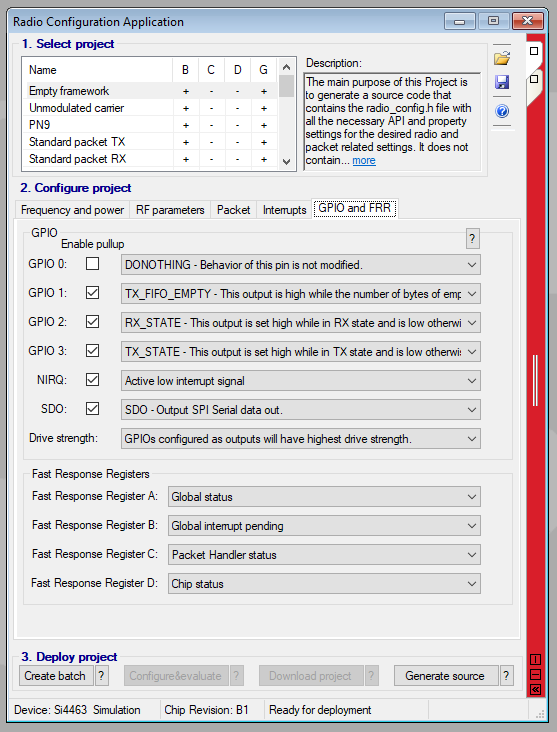
\includegraphics[width=0.75\textwidth]{figures/wds-tutorial-14.png}
		\caption{Step 14 of the radio configuration.}
		\label{fig:wds-tutorial-step-14}
	\end{center}
\end{figure}

\subsection{Step 15}

\begin{enumerate}
    \item Click in ``Generate Source" and select the ``.h" type of source.
    \item The software will ask where to save the generated file.
    \item The generated *.h file must be copied to the directory of the rf4463 driver.
\end{enumerate}

\section{Final Remarks}

This tutorial has the objective of generate a basic configuration parameters of the radio, some functionalities of the radio are not covered by the WDS software, and so, must be configured/controlled in the device driver.

\chapter{Compiling and Building the Beacon Firmware}

This tutorial is a reference to compile, build and flash the firmware of the beacon of the TTC module. All the software development was made using the Code Composer Studio (CCS) IDE, version 7.3.0. To load the code into the TTC MCU, the MSP-FET can be used.

\section{Creating the Project}

After the download and installation of the CCS, open it and create a new project with following steps:

\begin{enumerate}
    \item Go to ``File" -> ``New" -> ``CCS Project".
    \item The window from the figure \ref{fig:compiling-tutorial} will appear on the screen.
    \item On ``Target", select MSP430F6659.
    \item On ``Project name", enter the name of the project (It can be ``beacon", ``beacon\_firmware", or whatever name you want).
    \item On ``Project templates and examples" box, select ``Empty project".
    \item Click on ``Finish".
\end{enumerate}

\begin{figure}[!h]
	\begin{center}
		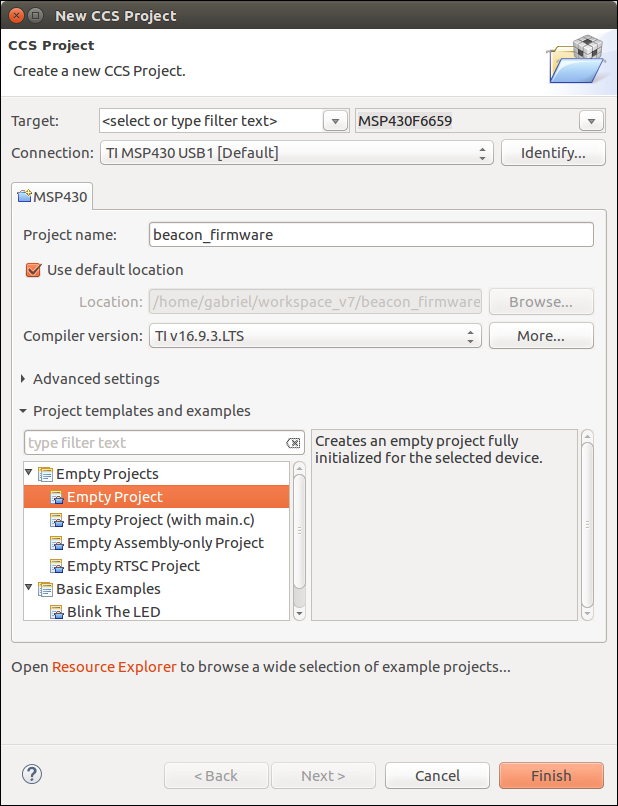
\includegraphics[width=0.75\textwidth]{figures/ccs_project.png}
		\caption{New CCS project window.}
		\label{fig:compiling-tutorial}
	\end{center}
\end{figure}

Now the beacon project with the correct parameters has been created, and the project source code files must be moved to the project directory. Copy the files inside the ``beacon" folder from the TTC git repository to the project folder.

\section{Compiling and Building}

To compile and build the firmware, click on "Project" -> "Build Project". If the process finish with no errors, the code is ready to go to the MCU of the beacon.

\section{Flashing}

To load the code into the board, connect the MSP-FET in the computer and follow the power-on tutorial.

With the board turned on and the MSP-FET connected, click on ``Run" -> ``Debug" or just press F11. If no errors occur, the firmware was loaded succesfully to the board.

\chapter{Power-On the TTC Module}

To power-on the TTC module, there are three different possibilities:

\begin{enumerate}
    \item Using three different power sources: one for the MCU, one for the beacon radio module and one for the telemetry radio module.
    \item Using two different power sources: one for each radio module (in this case, the beacon MCU is powered using the JTAG bus).
    \item Using just one power source to all components (THIS METHOD IS NOT SAFE: there is no control over the power consumption of each component).
\end{enumerate}

To test just the beacon, there is no need to power-on the telemetry radio module. Turning on the telemetry radio only makes sense if an external module is connected and controlling it (Like an OBC or an OBDH).

The connections reference of the TTC board can be found in External Connections.

\section{Using an External Power Source for the Beacon MCU}

\subsection{Power-On the Beacon MCU}

\begin{enumerate}
    \item Set an output of a channel of the power source to $3,3\ V$ and $30\ mA$ (Cut-off current).
    \item Connect the positive cable to the H2A-14 or H2B-14 pin of the PCI-104 connector.
    \item Connect the ground cable to any GND pin of the PCI-104 connector.
    \item Turn on this channel of the power source.
\end{enumerate}

\subsection{Power-On the Beacon Radio Module}

\begin{enumerate}
    \item Set another output of a channel of the power source to $5,0\ V$ and $500\ mA$ (Cut-off current).
    \item Connect the positive cable to the H1A-26 pin of the PCI-104 connector.
    \item Connect the ground cable to any GND pin of the PCI-104 connector.
    \item Turn on this channel of the power source.
\end{enumerate}

\subsection{Power-On the Telemetry Radio Module}

\begin{enumerate}
    \item Set another output of a channel of the power source to $5,0\ V$ and $500\ mA$ (Cut-off current).
    \item Connect the positive cable to the H1A-25 pin of the PCI-104 connector.
    \item Connect the ground cable to any GND pin of the PCI-104 connector.
    \item Turn on this channel of the power source.
\end{enumerate}

\section{Using the JTAG as Power Source for the Beacon MCU}

In this case, to power on the beacon MCU, just connect a jumper in the P4 connector of the board and after, connect a MSP-FET debbuger to the JTAG connector.

The procedure to power-on the radio modules is the same as above.

\chapter{Receiving the Beacon Data}

\section{Required Softwares}

\begin{itemize}
    \item GQRX (For just receive the signal).
    \item RTL-SDR drivers (The GRQX will install all the required drivers).
    \item FloripaSat GRS (For receive the signal and data).
\end{itemize}

\subsection{Supported SDRs}

\begin{itemize}
    \item RTL-SDR
    \item FunCube Dongle Pro+
\end{itemize}

\section{Receiving the Beacon Signal}

In this method, you will not be able to see the beacon data in real time. This only shows the presence of the beacon signals in the air.

The instructions to receive the beacon signal in the GQRX are available bellow:

\begin{enumerate}
    \item Open the GQRX software.
    \item Configure it for your SDR model.
    \item Press the power button on the upper left corner.
    \item Select the frequency to 145,9 MHz.
    \item Wait the spectrum of the beacon signal appear.
\end{enumerate}

The figure \ref{fig:beacon-signal-gqrx} illustrates the reception of the beacon signal in the GQRX software.

\begin{figure}[!h]
	\begin{center}
		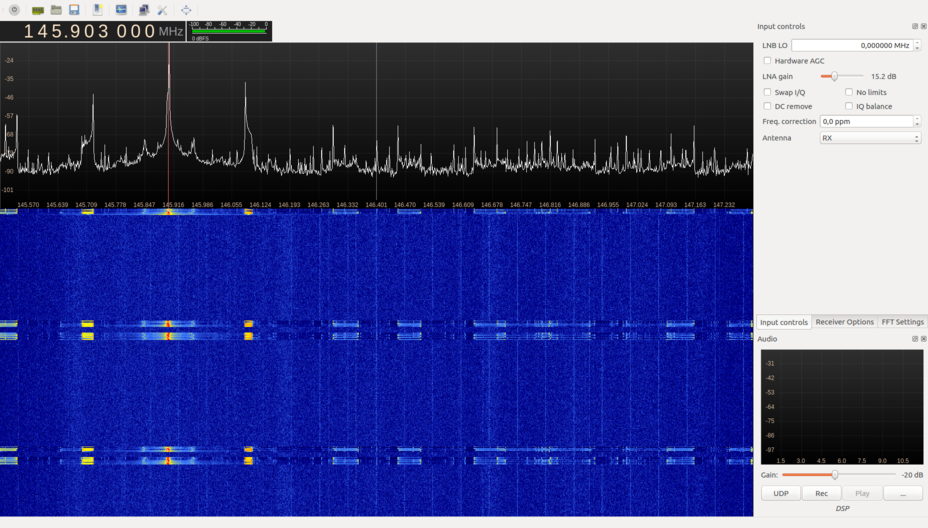
\includegraphics[width=\textwidth]{figures/beacon-signal-gqrx.png}
		\caption{Beacon signal in GQRX.}
		\label{fig:beacon-signal-gqrx}
	\end{center}
\end{figure}

\section{Receiving the Beacon Data}

Using this method, you will be able to see the beacon (and the telemetry) data in real time on the computer screen. For that, the FloripaSat GRS sofware is required.

\begin{enumerate}
    \item Open the FloripaSat GRS software.
    \item Connect a the SDR device.
    \item Select the source of the signal.
    \item Press the play button in the beacon frame.
    \item A new window will appear in the screen, with the FFT and Waterfall plot of the received signal (in real time) of the connected SDR.
    \item Power on the beacon module of the TTC board.
    \item Adjust the frequency of the receive to the center frequency of the beacon signal (Use the FFT and the Waterfall plot for that).
    \item With the correct frequency sinthonization, the beacon data should appear in the main window of the FloripaSat GRS softwate.
\end{enumerate}

\begin{figure}[!h]
	\begin{center}
		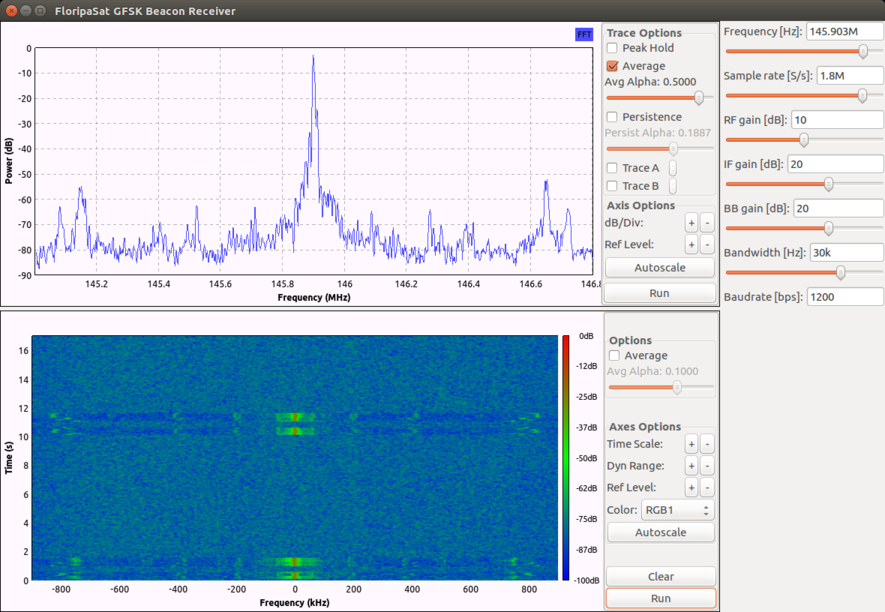
\includegraphics[width=\textwidth]{figures/beacon-signal-gnuradio.png}
		\caption{Beacon signal in the GNURadio receiver from the FloripaSat GRS.}
		\label{fig:beacon-signal-gnuradio}
	\end{center}
\end{figure}

\begin{figure}[!h]
	\begin{center}
		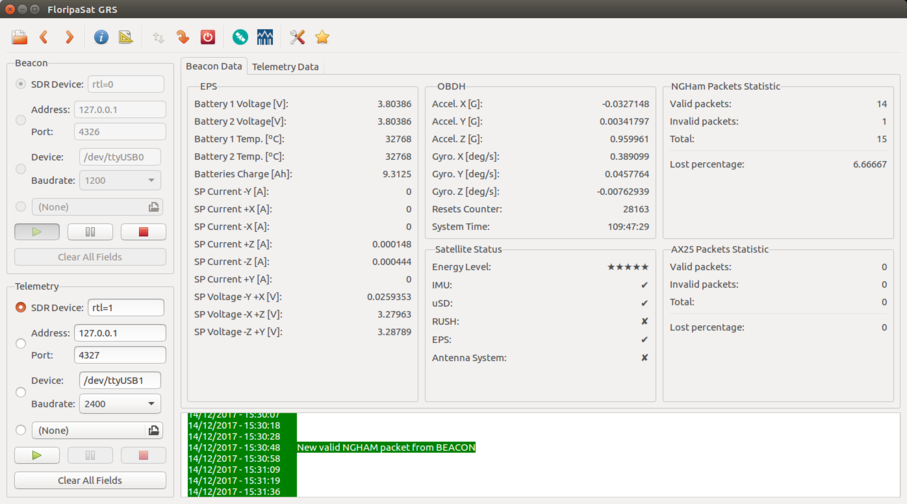
\includegraphics[width=\textwidth]{figures/beacon-data-grs.png}
		\caption{Beacon data in the FloripaSat GRS.}
		\label{fig:beacon-data-grs}
	\end{center}
\end{figure}

\end{appendices}

\end{document}
